%%%%%%%%%%%%%%%%%%%%%%%%%%%%%%
%
% $Autor: Wings $
% $Datum: 2019-12-09 11:50:02Z $
% $Pfad: komponenten/Bilderkennung/Produktspezifikation/CorelTPU/TPU/Allgemein/tikzdefs.tex $
% $Version: 1766 $
%
%
%%%%%%%%%%%%%%%%%%%%%%%%%%%%%%


% Definition für tikz

\usepackage{pgfplots}
\usepackage{pgf,tikz}
\usepackage{mathrsfs}
\usepackage{circuitikz}
\usepackage{tikz}
\usetikzlibrary{shapes,shapes.symbols,shapes.misc, shapes.multipart, shapes.geometric,arrows,angles,quotes,babel,positioning,calc,math,matrix,backgrounds}
\usetikzlibrary{positioning,fadings,through}
\usetikzlibrary{math}


\usepackage{tikz-3dplot}

\definecolor{ArduinoColor}{rgb}{0.1,0.5,0.6}
\definecolor{BlackGreen}{rgb}{0.5, 0.68,0.375}
\definecolor{Or}{rgb}{0.945, 0.768,0.0588}
\definecolor{Cyann}{rgb}{0.1,0.9,0.9}
\definecolor{DarkOrange}{rgb}{0.89, 0.4,0.09}


\tikzset{
  input2/.style={ % requires library shapes.geometric
    draw,
    trapezium,
    trapezium left angle=60,
    trapezium right angle=120,
  },
  process rectangle outer width/.initial=0.15cm,
  predefined process/.style={
    rectangle,
    draw,
    append after command={
      \pgfextra{
        \draw [fill=blue!20]
        ($(\tikzlastnode.north west)-(0,0.5\pgflinewidth)$)--
        ($(\tikzlastnode.north west)-(\pgfkeysvalueof{/tikz/process rectangle outer width},0.5\pgflinewidth)$)--
        ($(\tikzlastnode.south west)+(-\pgfkeysvalueof{/tikz/process rectangle outer width},+0.5\pgflinewidth)$)--
        ($(\tikzlastnode.south west)+(0,0.5\pgflinewidth)$);
        \draw [fill=blue!20]
        ($(\tikzlastnode.north east)-(0,0.5\pgflinewidth)$)--
        ($(\tikzlastnode.north east)+(\pgfkeysvalueof{/tikz/process rectangle outer width},-0.5\pgflinewidth)$)--
        ($(\tikzlastnode.south east)+(\pgfkeysvalueof{/tikz/process rectangle outer width},0.5\pgflinewidth)$)--
        ($(\tikzlastnode.south east)+(0,0.5\pgflinewidth)$);
      }  
    },
    text width=#1,
    align=center, fill=blue!20,  minimum height=4em
  },
  predefined process/.default=20mm,
  data1/.style={
    trapezium, 
    trapezium left angle=70, 
    trapezium right angle=110, 
    text width=1.5cm, 
    inner ysep=17pt,
    align=center, 
    line width=2pt,
    fill=blue!20
  },      
}


%Kabinettprojektion von 3D auf 2D
%
% Eingabe
% x,y,z
%
% Ausgabe
% x- oder y-Wert des Punkts
\newcommand{\Proj}[3]{({#1-#3*0.5*cos(30)},{#2-#3*0.5*sin(30)})}
\tikzset{declare function={ProjX(\x,\y,\z)=\x-\z*0.5*cos(30);}}
\tikzset{declare function={ProjY(\x,\y,\z)=\y-\z*0.5*sin(30);}}

%Rotation um die x-Achse 
%
% Eingabe
% x,y,z,alpha
%
% Ausgabe
% 
% x-, y- oder z-Wert des Punkts
\tikzset{declare function={RotXx(\x,\y,\z,\a)=\x;}}
\tikzset{declare function={RotXy(\x,\y,\z,\a)=\y*cos(\a)-\z*sin(\a);}}
\tikzset{declare function={RotXz(\x,\y,\z,\a)=\y*sin(\a)+\z*cos(\a);}}


%Rotation um die y-Achse 
%
% Eingabe
% x,y,z,alpha
%
% Ausgabe
% 
% x-, y- oder z-Wert des Punkts
\tikzset{declare function={RotYx(\x,\y,\z,\a)=\x*cos(\a)-\z*sin(\a);}}
\tikzset{declare function={RotYy(\x,\y,\z,\a)=\y;}}
\tikzset{declare function={RotYz(\x,\y,\z,\a)=\x*sin(\a)+\z*cos(\a);}}



%Rotation um die z-Achse 
%
% Eingabe
% x,y,z,alpha
%
% Ausgabe
% 
% x-, y- oder z-Wert des Punkts
\tikzset{declare function={RotZx(\x,\y,\z,\a)=\x*cos(\a)-\y*sin(\a);}}
\tikzset{declare function={RotZy(\x,\y,\z,\a)=\x*sin(\a)+\y*cos(\a);}}
\tikzset{declare function={RotZz(\x,\y,\z,\a)=\z;}}


%Rotation um die x-Achse 
%
% Eingabe
% x,y,z,alpha
%
% Ausgabe
% Punkt {x}{y}{z}
\newcommand{\RotXx}[4]{#1}%
\newcommand{\RotXy}[4]{(cos(#4)*#2-sin(#4)*#3)}
\newcommand{\RotXz}[4]{(sin(#4)*#2+cos(#4)*#3)}%


\tikzset{declare function={bellshape(\x,\mu,\sigma)=exp(-(\x-\mu)^2/(2*\sigma^2));}}


%Rotation um die x-Achse mit Projektion
%
% Eingabe
% x,y,z,alpha
%
% Ausgabe
% Punkt ({x}, {y})
\newcommand{\RotXP}[4]%
{(%
{#1-(sin(#4)*#2+cos(#4)*#3)*0.5*cos(30)},%
{cos(#4)*#2-sin(#4)*#3-(sin(#4)*#2+cos(#4)*#3)*0.5*sin(30)})%
}

%Rotation um die y-Achse mit Projektion
%
% Eingabe
% x,y,z,alpha
%
% Ausgabe
% Punkt ({x}, {y})
\newcommand{\RotYP}[4]%
{(%
{cos(#4)*#1+sin(#4)*#3-(-sin(#4)*#1+cos(#4)*#3)*0.5*cos(30)},%
{#2-(-sin(#4)*#1+cos(#4)*#3)*0.5*sin(30)}%
)}


%Rotation um die z-Achse mit Projektion
%
% Eingabe
% x,y,z,alpha
%
% Ausgabe
% Punkt ({x}, {y})
\newcommand{\RotZP}[4]%
{({cos(#4)*#1-sin(#4)*#2-#3*0.5*cos(30)},{sin(#4)*#1+cos(#4)*#2-#3*0.5*sin(30)})}


% Parameter
% #1: Skalierung
% #2: Winkel; 0..179
\newcommand{\HermiteSymPSP}[2]{%
  \pgfmathsetmacro{\RADIUS}{6}
  
  \begin{scope}[scale=#1]
    
    % angle 
    \begin{scope}[shift={(\RADIUS,0cm)}]
      \draw[fill=green!30] (0,0) -- (180:0.25*\RADIUS) arc (180:#2:0.25*\RADIUS);
      \draw ({0.5*(180+#2)}:{0.175*\RADIUS}) node {$\beta$};
      \draw ({0.5*(#2)}:{0.175*\RADIUS}) node {$\alpha$}; %$\pi-\alpha$
    \end{scope}
    
    \coordinate[label=left:$P_0$]  (P0) at (0,0);
    \coordinate  (t0) at (0.25*\RADIUS,0);
    \coordinate[label=below:$S$]  (S) at (\RADIUS,0);
    \coordinate  (s0) at (1.3*\RADIUS,0);
    \coordinate[label=left:$P_1$] (P1) at ({\RADIUS+\RADIUS*cos(#2)},{\RADIUS*sin(#2)});
    
    \draw [black,line width=0.5pt,domain=0:#2,->] plot ({\RADIUS+0.25*\RADIUS*cos(\x)}, {0+0.25*\RADIUS*sin(\x)});
    
    \draw [line width=1.5pt] (P0) -- (S) --(P1);
    \draw [line width=0.2pt,dotted] (S) --(s0);
    \node (P00) at (P0) {$\bullet$};
    \node (P11) at (P1) {$\bullet$};
  \end{scope}
}


% Parameter
% #1: Skalierung
% #2: Winkel; 0..179
\newcommand{\HermiteSym}[2]{%
   \pgfmathsetmacro{\RADIUS}{6}
  
   \begin{scope}[scale=#1]

     % angle 
     \begin{scope}[shift={(\RADIUS,0cm)}]
       \draw[fill=green!30] (0,0) -- (180:0.25*\RADIUS) arc (180:#2:0.25*\RADIUS);
       \draw ({0.5*(180+#2)}:{0.175*\RADIUS}) node {$\beta$};
       \draw ({0.5*(#2)}:{0.175*\RADIUS}) node {$\alpha$}; %$\pi-\alpha$
     \end{scope}

     \coordinate[label=left:$P_0$]  (P0) at (0,0);
     \coordinate  (t0) at (0.25*\RADIUS,0);
     \coordinate[label=below:$S$]  (S) at (\RADIUS,0);
     \coordinate  (s0) at (1.3*\RADIUS,0);
     \coordinate[label=left:$P_1$] (P1) at ({\RADIUS+\RADIUS*cos(#2)},{\RADIUS*sin(#2)});
     \coordinate (t1) at ({\RADIUS+ 1.25*\RADIUS*cos(#2)},{1.25*\RADIUS*sin(#2)});
  
     \coordinate[label=below:$\vec{t}_0$](T0) at ($ (P0)!.5!(t0) $);
     \coordinate[label=right:$\vec{t}_1$](T1) at ($ (P1)!.5!(t1) $);

     \draw [black,line width=0.5pt,domain=0:#2,->] plot ({\RADIUS+0.25*\RADIUS*cos(\x)}, {0+0.25*\RADIUS*sin(\x)});

     \draw [line width=1.5pt] (P0) -- (S) --(P1);
     \draw [line width=2pt,->,color=red] (P0) -- (t0);
     \draw [line width=2pt,->,color=red] (P1) -- (t1);
     \draw [line width=0.2pt,dotted] (S) --(s0);
     \node (P00) at (P0) {$\bullet$};
     \node (P11) at (P1) {$\bullet$};
  \end{scope}
}


% Parameter
% #1: Skalierung
% #2: Winkel; 0..-179
\newcommand{\HermiteSymNeg}[2]{%
  \pgfmathsetmacro{\RADIUS}{6}
  
  \begin{scope}[scale=#1]
    
    % angle 
    \begin{scope}[shift={(\RADIUS,0cm)}]
      \draw[fill=green!30] (0,0) -- (-180:0.25*\RADIUS) arc (-180:#2:0.25*\RADIUS);
      \draw ({0.5*(-180+#2)}:{0.175*\RADIUS}) node {$\beta$};
      \draw ({0.5*(#2)}:{0.175*\RADIUS}) node {$\alpha$}; %$\pi-\alpha$
    \end{scope}
    
    \coordinate[label=left:$P_0$]  (P0) at (0,0);
    \coordinate  (t0) at (0.25*\RADIUS,0);
    \coordinate[label=above:$S$]  (S) at (\RADIUS,0);
    \coordinate  (s0) at (1.3*\RADIUS,0);
    \coordinate[label=left:$P_1$] (P1) at ({\RADIUS+\RADIUS*cos(#2)},{\RADIUS*sin(#2)});
    \coordinate (t1) at ({\RADIUS+ 1.25*\RADIUS*cos(#2)},{1.25*\RADIUS*sin(#2)});
    
    \coordinate[label=below:$\vec{t}_0$](T0) at ($ (P0)!.5!(t0) $);
    \coordinate[label=right:$\vec{t}_1$](T1) at ($ (P1)!.5!(t1) $);
    
    \draw [black,line width=0.5pt,domain=0:#2,->] plot ({\RADIUS+0.25*\RADIUS*cos(\x)}, {0+0.25*\RADIUS*sin(\x)});
    
    \draw [line width=1.5pt] (P0) -- (S) --(P1);
    \draw [line width=2pt,->,color=red] (P0) -- (t0);
    \draw [line width=2pt,->,color=red] (P1) -- (t1);
    \draw [line width=0.2pt,dotted] (S) --(s0);
    \node (P00) at (P0) {$\bullet$};
    \node (P11) at (P1) {$\bullet$};
  \end{scope}
}

\tikzstyle{bigblock} = [draw, fill=blue!20, rectangle, minimum height=1.5em, minimum width=8em]
\tikzstyle{mediumblock} = [draw, fill=red!20, rectangle, minimum height=1.5em, minimum width=4em]
\tikzstyle{smallblock} = [draw, fill=red!20, rectangle, minimum height=1.5em, minimum width=1.5em]
\tikzstyle{arrow} = [->,shorten >=1pt,>=stealth',semithick]

\definecolor{LightCyan}{rgb}{0.88,1,1}
\definecolor{frenchblue}{rgb}{0.0, 0.45, 0.73}
\definecolor{greenblue}{rgb}{0.0, 0.25, 0.3}
\definecolor{darkcyan}{rgb}{0.0, 0.55, 0.55}
\definecolor{bondiblue}{rgb}{0.0, 0.58, 0.71}
\definecolor{grayleft}{rgb}{0.1, 0.1, 0.1}
\definecolor{grayright}{rgb}{0.2, 0.2, 0.2}
\definecolor{graycircle}{rgb}{0.3, 0.3, 0.3}
\definecolor{graylight}{rgb}{0.8, 0.8, 0.8}
\definecolor{greenenglish}{rgb}{0.0, 0.5, 0.0}
\definecolor{darkpastelgreen}{rgb}{0.01, 0.75, 0.24}
\definecolor{copper}{rgb}{0.72, 0.45, 0.2}
\definecolor{greenyellow}{rgb}{0.68, 1.0, 0.18}
\definecolor{fuchsia}{rgb}{1.0, 0.0, 1.0}
\definecolor{silver}{rgb}{0.75, 0.75, 0.75}
\definecolor{deepskyblue}{rgb}{0.0, 0.75, 1.0}

% Beispiele
%
%\begin{center}
%  \begin{tikzpicture}
%  \HermiteSym{1}{120}
%  \end{tikzpicture}
%\end{center}
%
%\begin{center}
%  \begin{tikzpicture}
%  \HermiteSym{1}{70}
%  \end{tikzpicture}
%\end{center}
%
%\begin{center}
%  \begin{tikzpicture}
%  \HermiteSym{1}{20}
%  \end{tikzpicture}
%\end{center}
%
%\begin{center}
%  \begin{tikzpicture}
%  \HermiteSym{1}{0}
%  \end{tikzpicture}
%\end{center}
%
%
%\begin{center}
%  \begin{tikzpicture}
%  \HermiteSymNeg{1}{-20}
%  \end{tikzpicture}
%\end{center}
%
%\begin{center}
%  \begin{tikzpicture}
%  \HermiteSymNeg{1}{-70}
%  \end{tikzpicture}
%\end{center}
%
%
%\begin{center}
%  \begin{tikzpicture}
%  \HermiteSymNeg{1}{-120}
%  \end{tikzpicture}
%\end{center}
%

%tikz-Kommandos

% Basis eines Roboters
% #1: Drehung des Systems
% #2: X-Offset des gedrehten Systems
% #3: Y-Offset des gedrehten Systems
% #4: Skalierung
\newcommand{\BASE}[4]{
  \begin{scope}[rotate=#1,scale=#4]  
    
    \draw[ultra thick, black]   ({#2-0.5},{#3-0.7}) -- ({#2+0.5},{#3-0.7});
    \draw[ultra thick, black]   ({#2-0.3},{#3-0.7}) -- ({#2-0.5},{#3-0.9});    
    \draw[ultra thick, black]   ({#2-0.1},{#3-0.7}) -- ({#2-0.3},{#3-0.9});    
    \draw[ultra thick, black]   ({#2+0.1},{#3-0.7}) -- ({#2-0.1},{#3-0.9});    
    \draw[ultra thick, black]   ({#2+0.3},{#3-0.7}) -- ({#2+0.1},{#3-0.9});    
    \draw[ultra thick, black]   ({#2+0.5},{#3-0.7}) -- ({#2+0.3},{#3-0.9});    
    
    \draw[thick, fill=blue!20]   ({#2-0.25},{#3-0.7}) -- ({#2+0.25},{#3-0.7}) -- ({#2},{#3}) -- ({#2-0.25},{#3-0.7});
    \draw[black, thick, fill=black]  (#2,#3) ellipse (0.1 and 0.1);
  \end{scope}
}%  


% Drehgelenk eines Roboters
% #1: Drehung des Gelenks
% #2: X-Offset des Systems
% #3: Y-Offset des Systems
% #4: Skalierung
\newcommand{\LINK}[4]{
  \begin{scope}[scale=#4]
    \draw[green, thick, fill=green!20]  ({#2+0.0},{#3+0.0}) ellipse (0.2 and 0.2);
    \draw[green, thick, fill=green!20]  ({#2+2.0*cos(#1)},{#3+2.0*sin(#1)}) ellipse (0.2 and 0.2);
    \draw[green!20, thick, fill=green!20]
    ({#2+0+0.2*cos(90+#1)},{#3+0+0.2*sin(90+#1)})
    --
    ({#2+2.0*cos(#1)+0.2*cos(90+#1)},{#3+2.0*sin(#1)+0.2*sin(90+#1)})
    --
    ({#2+2.0*cos(#1)+0.2*cos(-90+#1)},{#3+2.0*sin(#1)+0.2*sin(-90+#1)})
    --
    ({#2+0+0.2*cos(-90+#1)},{#3+0+0.2*sin(-90+#1)})
    --
    ({#2+0+0.2*cos(90+#1)},{#3+0+0.2*sin(90+#1)});
    \draw[green, thick]
    ({#2+0+0.2*cos(90+#1)},{#3+0+0.2*sin(90+#1)})
    --
    ({#2+2.0*cos(#1)+0.2*cos(90+#1)},{#3+2.0*sin(#1)+0.2*sin(90+#1)});
    \draw[green, thick]
    ({#2+2.0*cos(#1)+0.2*cos(-90+#1)},{#3+2.0*sin(#1)+0.2*sin(-90+#1)})
    --
    ({#2+0+0.2*cos(-90+#1)},{#3+0+0.2*sin(-90+#1)});
    \draw[black, thick, fill=blue]  ({#2+0.0},{#3+0.0}) ellipse (0.1 and 0.1);
    \draw[black, thick, fill=black]  ({#2+2*cos(#1)},{#3+2*sin(#1)}) ellipse (0.1 and 0.1);
    
  \end{scope}
}%  

% Drehgelenk eines Roboters
% #1: 1.Punkt x
% #2: 1.Punkt y
% #3: 2.Punkt x
% #4: 2.Punkt y
\newcommand{\LINKP}[4]{
  \begin{scope}
     \tikzmath{
       \Px  = #1;
       \Py  = #2;
       \Qx  = #3;
       \Qy  = #4;
       \Dx   = \Qx-\Px;
       \Dy   = \Qy-\Py;
       \Winkel = 45;
       \Pp  = \Dy*pow(\Dx,-1);
       \Winkel = atan(\Pp);
       \Laenge = pow(pow(\Dx,2)+pow(\Dy,2),0.5);
     }    
    
  
    \LINK{\Winkel}{#1}{#2}{1}
  \end{scope}
}%  

% SCARA-Roboters
% #1: Drehung des Systems
% #2: X-Offset des gedrehten Systems
% #3: Y-Offset des gedrehten Systems
% #4: Winkel des 1.Gelenks
% #5: Winkel des 2.Gelenks
% #6: Skalierung
% #7: Auswahl ungerade mit Beschriftung der Armlängen 
%           2 und 3: mit Winkel

\newcommand{\SCARA}[7]{
  \def\Rot{#1}
  \def\OffsetX{#2}
  \def\OffsetY{#1}
  \def\Alpha{#4}
  \def\Beta{#5}
  \def\Auswahl{#7}
  
  \begin{scope}[scale=#6]
    \BASE{\Rot}{\OffsetX}{\OffsetY}{1}
    \LINK{\Alpha}{\OffsetX}{\OffsetY}{1}
    \LINK{\Beta}{\OffsetX+2*cos(\Alpha)}{\OffsetY+2*sin(\Alpha)}{1}
    
    \ifthenelse{\isodd{\Auswahl}}
    {
        \node (Q1T) at (\OffsetX-0.6,\OffsetY) {$(0,0)$};
        \node (Q2T) at ({\OffsetX+1*cos(\Alpha)-0.4*sin(\Alpha)},{\OffsetY+1*sin(\Alpha)+0.4*cos(\Alpha)}) {$\ell_1$};
        \node (Q3T) at ({\OffsetX+2*cos(\Alpha)+1*cos(\Alpha+\Beta)+0.2*sin(\Alpha+\Beta)},{\OffsetY+2*sin(\Alpha)+1*sin(\Alpha+\Beta)-     0.2*cos(\Alpha+\Beta)}) {$\ell_2$};
    }{}    
    
    \ifthenelse{\equal{\Auswahl}{2}\or \equal{\Auswahl}{3}}
    {    
      \draw[color=red] ({cos(\Rot)*\OffsetX+sin(\Rot)*\OffsetY},
                       {-sin(\Rot)*\OffsetX+cos(\Rot)*\OffsetY})
              --
                    ({cos(\Rot)*(\OffsetX+1)+sin(\Rot)*\OffsetY},
                    {-sin(\Rot)*(\OffsetX+1)+cos(\Rot)*\OffsetY});
      \draw[color=red]
         ({cos(\Rot+\Alpha)*\OffsetX-sin(\Rot+\Alpha)*\OffsetY},
          {sin(\Rot+\Alpha)*\OffsetX+cos(\Rot+\Alpha)*\OffsetY})
          --
       ({cos(\Rot-\Alpha)*(\OffsetX+1)-sin(\Rot-\Alpha)*\OffsetY},
       {sin(\Rot+\Alpha)*(\OffsetX+1)+cos(\Rot+\Alpha)*\OffsetY});

      \draw[color=red] ({cos(\Rot)*(\OffsetX+2*cos(\Alpha))
                           +sin(\Rot)*(\OffsetY+2*sin(\Alpha))},
                       {-sin(\Rot)*(\OffsetX+2*cos(\Alpha))+cos(\Rot)*(\OffsetY+2*sin(\Alpha))})
              --
                    ({cos(\Rot+\Alpha)*((\OffsetX+2*cos(\Alpha))+1)+sin(\Rot+\Alpha)*(\OffsetY+2*sin(\Alpha))},
                    {-sin(\Rot-\Alpha)*((\OffsetX+2*cos(\Alpha))+1)+cos(\Rot-\Alpha)*(\OffsetY+2*sin(\Alpha))});

      \draw[color=red] ({cos(\Rot)*(\OffsetX+2*cos(\Alpha))
                           +sin(\Rot)*(\OffsetY+2*sin(\Alpha))},
                       {-sin(\Rot)*(\OffsetX+2*cos(\Alpha))+cos(\Rot)*(\OffsetY+2*sin(\Alpha))})
              --
                    ({cos(\Rot+\Alpha+\Beta)*((\OffsetX+2*cos(\Alpha))+1)+sin(\Rot+\Alpha+\Beta)*(\OffsetY+2*sin(\Alpha))},
                    {-sin(\Rot-\Alpha+\Beta)*((\OffsetX+2*cos(\Alpha))+1)+cos(\Rot-\Alpha+\Beta)*(\OffsetY+2*sin(\Alpha))});

    }{}    
  \end{scope}
}%  


% Nicht fertig
\newcommand{\SCARAXY}[6]{
  \begin{scope}[scale=#6]
    \def\ScaraX{#1}
    \def\ScaraY{#2}
    %ang2=90-(ACOS((L1^2-L2^2+x^2+y^2)/(2*L1*RAIZ(x^2+y^2)))+(ATAN(x/y))
    \def\ScaraTheta2{3.1415926*0.5-acos((sqrt(\ScaraX^2+\ScaraY^2)/4)+atan(\ScaraX/\ScaraY)}
    %angB=180-ACOS((L1^2+L2^2-x^2-y^2)/(2*L1*L2))
    \def\AngleB{3.1415926-acos((8-\ScaraX^2-\ScaraY^2)/8}
    % ang1=ang2+angB
    \def\ScaraTheta2{\ScaraTheta2+\AngleB}
  \end{scope}
}%  

% Planarer Roboter mit 3 Links
% #1: Drehung des Systems
% #2: X-Offset des gedrehten Systems
% #3: Y-Offset des gedrehten Systems
% #4: Winkel des 1.Gelenks
% #5: Winkel des 2.Gelenks
% #6: Winkel des 3.Gelenks
% #6: Skalierung

\newcommand{\RRRPLANAR}[7]{
  \def\Rot{#1}
  \def\OffsetX{#2}
  \def\OffsetY{#1}
  \def\Alpha{#4}
  \def\Beta{#5}
  \def\Gamma{#6}
  
  \begin{scope}[scale=#7]
    \BASE{\Rot}{\OffsetX}{\OffsetY}{1}
    \LINK{\Alpha}{\OffsetX}{\OffsetY}{1}
    \LINK{\Beta}{\OffsetX+2*cos(\Alpha)}{\OffsetY+2*sin(\Alpha)}{1}
    \LINK{\Gamma}{\OffsetX+2*cos(\Alpha)+2*cos(\Beta)}{\OffsetY+2*sin(\Alpha)+2*sin(\Beta)}{1}
  \end{scope}
}%  
    


% Kreisbogen
%\draw [green,line width=0.5pt,domain=0:180] plot ({5+1*cos(\x)}, {3+1*sin(\x)});


\newcommand{\tstar}[5]{% inner radius, outer radius, tips, rot angle, options
  \pgfmathsetmacro{\starangle}{360/#3}
  \draw[#5] (#4:#1)
  \foreach \x in {1,...,#3}
  { -- (#4+\x*\starangle-\starangle/2:#2) -- (#4+\x*\starangle:#1)
  }
  -- cycle;
}


\newcommand{\ngram}[4]{% outer radius, tips, rot angle, options
  \pgfmathsetmacro{\starangle}{360/#2}
  \pgfmathsetmacro{\innerradius}{#1*sin(90-\starangle)/sin(90+\starangle/2)}
  \tstar{\innerradius}{#1}{#2}{#3}{#4}
}


% Zeichnen der Scherenkinematik
% Die ersten Parameter sind X und Y-Position
% Der dritte Parameter zeigt gegebenenfalls Bezeichnungen:
% 0 : Keine Bezeichnung
% 1 : Veränderliche Parameter
% 2 : Konstrukvie Parameter
% 3 : Alle Parameter
\newcommand{\Scissor}[3]%
{
  \begin{center}
    \begin{tikzpicture}
      \def\ScissorX{#1}
      \def\ScissorY{#2}
      \def\Auswahl{#3}
    
      \tikzmath{\HF  =  8; % Rahmenhoehe
                \DF  = 12.5; % Rahmenbreite
                \BF  = 0.2; % Breite der Balken
                \Arm = 6;   % Länge des Arms
                \DS  = 0.6; % Breite der Zange
                \HS  = 0.3; % Höhe der Zange
                \PLx = \ScissorX-0.5*\DS;
                \PRx = \ScissorX+0.5*\DS;
                \Py  = \HF-\ScissorY+\HS;                
                \QL  = \PLx-pow(\Arm*\Arm-pow(\ScissorY-\HS,2),0.5); 
                \QR  = \PRx+pow(\Arm*\Arm-pow(\ScissorY-\HS,2),0.5);
               }
%               
      \draw[thick=4pt,fill] 
              (-\BF,0) -- (0,0) -- (0,\HF) -- (\DF,\HF) -- (\DF,0) -- (\DF+\BF,0) 
              -- (\DF+\BF,\HF+\BF) -- (-\BF,\HF+\BF) -- (-\BF,0);
      
      \draw[thick=2pt,red] 
         (\QL,{\HF+0.5*\BF}) -- (\PLx,\Py) -- (\PRx, \Py) -- (\QR,{\HF+0.5*\BF});
      \draw[thick=2pt,red,fill] 
            (\PLx,\Py) -- (\PRx, \Py) -- ({\ScissorX},{\HF-\ScissorY}) -- (\PLx,\Py);
       
      \draw [green,thick,domain=0:360,fill] plot ({\QL+0.5*\BF*cos(\x)}, {\HF+0.5*\BF+0.5*\BF*sin(\x)});
      \draw [green,thick,domain=0:360,fill] plot ({\QR+0.5*\BF*cos(\x)}, {\HF+0.5*\BF+0.5*\BF*sin(\x)});
      
      
      \draw [green,thick,domain=0:360,fill] plot ({\ScissorX+0.5*\BF*cos(\x)}, {\HF-\ScissorY+0.5*\BF+0.5*\BF*sin(\x)});
     
      \draw [green,thick,domain=0:360,fill] 
         plot (
                {\PLx+0.5*\BF*cos(\x)}, 
                {\Py+0.5*\BF*sin(\x)}
              );
      \draw [green,thick,domain=0:360,fill] 
        plot (
          {\PRx+0.5*\BF*cos(\x)}, 
          {\Py+0.5*\BF*sin(\x)}
        );
        
%        \LINK{-45}{\QL}{\HF}{1};

  \ifthenelse{\isodd{\Auswahl}}
  {
      \node (Q1T) at (\QL,\HF+\BF+0.3) {$q_l$};
      \node (Q2T) at (\QR,\HF+\BF+0.3) {$q_r$};
%      
  %Beschriftung
      \node (PL) at (\PLx-0.3,\Py) {$P_l$};
      \node (PR) at (\PRx+0.3,\Py) {$P_r$};
      \node (TCP) at (\ScissorX,\Py-0.3-\HS) {$(X,Y)$};
  }{}    
      
  \ifthenelse{\equal{\Auswahl}{2}\or \equal{\Auswahl}{3}}
  {
    % Konstruktive Parameter
      \draw (-\BF-0.3,0)  -- (-\BF-0.6,0);
      \draw (-\BF-0.3,\HF)  -- (-\BF-0.6,\HF);
      \draw[->]  ({-\BF-0.45},{\HF*0.5-0.3}) -- ({-\BF-0.45},0);
      \draw[->] ({-\BF-0.45},{\HF*0.5+0.3}) -- ({-\BF-0.45},{\HF}) ;
      \node (HF) at ({-\BF-0.45},{\HF*0.5+0.3}) {$\HFrame$};

      \draw[<-] (-\BF,\HF+\BF+0.6)  -- (0.5*\DF-0.3,\HF+\BF+0.6);      
      \draw[->] (0.5*\DF+0.3,\HF+\BF+0.6)  -- (\DF,\HF+\BF+0.6);      
      \node (DF) at (0.5*\DF,\HF+\BF+0.6)  {$\LFrame$};
 
      \draw [<->]  (\PLx-0.6,\Py)  -- (\PLx-0.6,{\Py-\HS});
      \node (HS) at  (\PLx-0.9,{\Py-0.5*\HS}) {$\HTongs$};

      \draw [<->]  (\PLx,\Py+0.3)  -- (\PRx,{\Py+0.3});
      \node (DS) at  (\ScissorX,{\Py+0.6}) {$\LTongs$};
 
     \draw[<->] (\QL -0.6,{\HF+0.5*\BF-0.6}) -- (\PLx-0.6,\Py-0.6);
     \node (LArm) at ({0.5*(\QL +\PLx)-0.9},{0.5*(\HF+0.5*\BF+\Py)-0.6}  ) {$\LArm$};
 }{}       
    \end{tikzpicture}
  \end{center}
}


\newcommand{\ArduinoNanoBLESense}[4]%
{
  \def\LowerLeftX{#1}
  \def\LowerLeftY{#2}
  \def\UpperRightX{#3}
  \def\UpperRightY{#4}
    
  \node at (0,0) (Board) {\includegraphics{Arduino/Nano33BLE/Nano33BLESense}};

  \fill[gray, opacity=0.7] (-6,-2.4) rectangle (6,2.4);

  \coordinate (A) at (\LowerLeftX,\LowerLeftY);
  \coordinate (B) at (\UpperRightX,\UpperRightY);    
  \begin{scope}
    \clip (A) rectangle (B);
    
    \node at (0,0) (Board) {\includegraphics{Arduino/Nano33BLE/Nano33BLESense}};
    
  \end{scope}
  \draw[yellow,line width=2pt] (A)  rectangle (B);
}


\newcommand{\ArduinoNanoTikz}{
    \begin{scope}[scale=1.5,rotate=90]
        \fill[ArduinoColor] (0,0) rectangle (3,7);
        \fill[gray!45] (0.85,6.35) rectangle++ (1.3,1);
        \foreach \y in {6.45,6.65,6.85,7.05,7.25}{
            \fill[gray!30,gray!30] (0.85,\y) rectangle ++(1.3, 0.1); }
        \foreach \x in {1.2,1.33125,1.4625,1.59375,1.725}{
            \draw[fill=gray!15,gray!15] (\x, 6.23) rectangle++ (0.075, 0.12); }
        \foreach \y  in{0.5,0.9,1.3,1.7,2.1,2.5,2.9,3.3,3.7,4.1,4.5,4.9,5.3,5.7,6.1} {
            \fill[gray!30] (0,\y) rectangle ++(0.25, 0.26); 
            \fill[gray!30] (2.75,\y) rectangle ++(0.25,0.26);}
        \foreach \y in {0.63,1.03,1.43,1.83,2.23,2.63,3.03,3.43,3.83,4.23,4.63,5.03,5.43,5.83,6.23} {
            \fill[gray!30](0.25,\y) circle (0.13);
            \fill[gray!30](2.75,\y) circle (0.13);
            \draw[fill=gray!60,gray!60](0.25,\y) circle (0.11);
            \draw[fill=gray!60,gray!60](2.75,\y) circle (0.11);
            \fill[white,white](0,\y) circle (0.085);
            \fill[white,white](3,\y) circle (0.085); }		
        \foreach \x in {0.2, 2.8} {
            \draw[fill=white!100,white!100](\x,0.2) circle (0.12);}
        \draw[fill=gray!60,gray!60] (1.1,5.1) rectangle++ (0.8,0.2);
        \draw[fill=gray!30, gray!30] (1.2,5) rectangle++(0.6,0.4);				
        \draw[fill=white, white] (1.5,5.2) circle (0.16) ;
        \draw[fill=gray!60,gray!60] (0.70, 0.55) rectangle (2.3,2.1);
        \fill[gray!45] (0.75, 0.6) rectangle (2.25,2.05);
        \foreach \x in {0.5,2.35}{
            \draw[fill=gray!15,gray!15] (\x,6.5) rectangle ++(0.12, 0.3); }
        \foreach \x in {0.56,2.4}{
            \draw[fill=Or, Or] (\x,6.65) circle(0.1); }
        \foreach \x in {0.2,2.8}{
            \draw[fill=white, white] (\x,6.8) circle(0.15); }
        \draw[fill=BlackGreen, BlackGreen] (0.7, 0) rectangle(2.3,0.55); 
        \draw[fill=black!100](0.5,2.8) rectangle++ (0.35,0.35);		
        \draw[fill=black!100](1.65,4) rectangle++ (0.3, 0.3);		
        \draw[fill=black!100](0.5,5.25) rectangle++ (0.35,0.5);
        \foreach \y in {2.25, 2.41}{
            \draw[fill=Cyann!70, Cyann!70] (1.85, \y) rectangle++(0.11, 0.11);
            \draw[fill=Cyann!70, Cyann!70] (2.01, \y) rectangle++(0.11, 0.11); }
        \draw[fill=gray!60, gray!60] (1.9,2.3) rectangle++(0.17, 0.17);
        
        \foreach \x in {0.85, 1}{
            \draw[fill=gray!30,gray!30](\x, 3.25) rectangle++(0.08, 0.18);
            \draw[fill=gray!60,gray!60](\x, 3.265) rectangle++(0.08, 0.15);}
        \draw[fill=gray!30,gray!30](1.12, 2.9) rectangle++(0.08, 0.18);		
        \draw[fill=gray!60, gray!60](1.12, 2.915) rectangle++(0.08, 0.15);
        
        \draw[fill=black, black] (1.26, 2.25) rectangle (1.66, 2.85);	
        \fill[white, white] (1.45, 2.4) circle(0.08);
        \fill[Or, Or] (1.45, 2.4) circle(0.06);
        \fill[white,white] (1.45, 2.4) circle(0.04);
        
        \draw[fill=black] (1.34,2.89) rectangle (1.66, 3.14);
        \draw[fill=black] (1.34,3.18) rectangle (1.66, 3.62);		
        \fill[white] (1.515, 3.5) circle(0.08);
        \fill[Or!30] (1.515, 3.5) circle(0.06);
        \draw[fill = black] (1.8, 3.1) rectangle(2.25, 3.62);
        
        \draw[fill=black] (0.5, 4.1) rectangle++ (0.8, 0.5);
        \foreach \x in {0.5714, 0.6928,0.8142,0.9357,1.0571,1.1782}{
            \draw[fill=gray!15,gray!15] (\x,4.05) rectangle++(0.05, 0.05);
            \draw[fill=gray!15,gray!15] (\x,4.6) rectangle++(0.05, 0.05);}
        \foreach \y in {4.16,4.27,4.38,4.49}{
            \draw[fill=gray!15,gray!15] (1.3,\y) rectangle++(0.05, 0.05); }
        \draw[fill=black] (1.6,5.6) rectangle++(0.25, 0.35); 
        \foreach \y in {5.65, 5.86}{
            \draw[fill=gray!45,gray!45] (1.47,\y) rectangle++(0.16, 0.04); 
            \draw[fill=gray!45,gray!45] (1.82,\y) rectangle++(0.16, 0.04);}
        
        \draw[fill=black] (2.05,5.5) rectangle++(0.24, 0.4); 
        \draw[fill=gray!30,gray!30] (2.15, 5.4) rectangle++(0.04, 0.15); 
        \draw[fill=gray!30,gray!30] (2.15,5.85) rectangle++(0.04, 0.15);
        
        \draw[rounded corners=2pt, fill=black] (1.15,5.6) rectangle++ (0.2,0.3);
        \foreach \y in {5.55, 5.85}{
            \fill[gray!45, opacity=0.7] (1.12,\y) rectangle++ (0.26, 0.1);}		
        \draw[rounded corners=2pt, fill=black] (2.1,4.4) rectangle++ (0.2,0.3);
        \foreach \y in {4.35, 4.65}{
            \fill[gray!45, opacity=0.8] (2.08,\y) rectangle++ (0.24, 0.1);}
        \foreach \y  in {4.35, 4.55}{
            \fill[gray!30,gray!30](1.7, \y) rectangle++ (0.22, 0.1);
            \fill[gray!60,gray!60](1.71, \y) rectangle++ (0.20, 0.1);}
        \draw[rounded corners=2pt, fill=black] (0.9,3.75) rectangle++ (0.3,0.2);
        \foreach \x in {0.85, 1.15}{
            \fill[gray!45, opacity=0.8] (\x,3.72) rectangle++ (0.1, 0.26);}		
        \foreach \y  in {2.6, 3.2, 3.4}{
            \draw[rounded corners=1pt, fill=gray!30,gray!30](0.5,\y) rectangle++ (0.2, 0.1); }
        \foreach \y  in {2.6, 3.2, 3.4}{		
            \draw [fill=gray!60,gray!60] (0.55, \y ) rectangle++ (0.1, 0.1); }
        
        \draw[rounded corners=1pt, fill=gray!30,gray!30](2.45,0.9) rectangle++ (0.1, 0.2);
        \draw [fill=gray!60, gray!60] (2.45, 0.95 ) rectangle++ (0.1, 0.1);
        
        \foreach \y in {0.2, 0.5}{
            \draw[rounded corners=1pt, fill=gray!30,gray!30] (0.5,\y) rectangle++ (0.1,0.2);}
        \foreach \y in {0.25, 0.55}{
            \draw [fill=gray!60,gray!60] (0.5, \y) rectangle++ (0.1, 0.1);}
        \draw [fill=gray!30,gray!30] (0.5, 1.7) rectangle++ (0.1, 0.2);
        \draw [fill=gray!60,gray!60] (0.5, 1.72) rectangle++ (0.1, 0.16);
        \foreach \x in {1.7, 2.2}{
            \draw[rounded corners=1pt, fill=gray!30,gray!30] (\x, 2.25 ) rectangle++ (0.1,0.2);}
        \foreach \x in {1.7, 2.2}{
            \draw [fill=gray!60,gray!60] (\x,2.3) rectangle++ (0.1, 0.1);}
        \draw[rounded corners=1pt, fill=gray!30, gray!30](2,2.7) rectangle++ (0.2,0.1);
        \draw [fill=gray!60,gray!60] (2.05,2.7) rectangle++ (0.1, 0.1);
        \foreach \x in {2, 2.2}{
            \draw[rounded corners=1pt, fill=gray!30,gray!30] (\x,5.1) rectangle++ (0.1,0.2);}
        \foreach \x in {2, 2.2}{
            \draw [fill=gray!60,gray!60] (\x,5.15) rectangle++ (0.1, 0.1);}
        
        \draw[rounded corners=1pt, fill=gray!30,gray!30] (0.6,6.0) rectangle++ (0.1,0.2);
        \draw [fill=gray!60,gray!60] (0.6,6.05) rectangle++ (0.1, 0.1);
        \draw[rounded corners=1pt, fill=gray!30,gray!30] (0.95,5.5) rectangle++ (0.1,0.2);
        \draw [fill=gray!60,gray!60] (0.95,5.55) rectangle++ (0.1, 0.1);
        \draw [fill=gray!30,gray!30] (0.7,5.85) rectangle++ (0.2, 0.1);
        \draw [fill=gray!60,gray!60] (0.72,5.85) rectangle++ (0.16, 0.1);
        
        \draw[rounded corners=1pt, fill=gray!30,gray!30] (2.5,6.2) rectangle++ (0.1,0.2);
        \draw [fill=gray!60,gray!60] (2.5,6.25) rectangle++ (0.1, 0.1);
        \draw[rounded corners=1pt, fill=gray!30,gray!30] (2.3,3.85) rectangle++ (0.1,0.2);
        \draw [fill=gray!60,gray!60] (2.3,3.9) rectangle++ (0.1, 0.1);
        \draw[rounded corners=1pt, fill=gray!30, gray!30] (2.15,4) rectangle++ (0.1,0.2);
        \draw [fill=gray!60,gray!60] (2.15,4.05) rectangle++ (0.1, 0.1);		
        
        \draw[rounded corners=1pt, fill=gray!30, gray!30](1.4,3.75)  rectangle++ (0.2,0.1);
        
        \draw [fill=gray!60,gray!60] (1.45,3.75) rectangle++ (0.1, 0.1);
        
        \draw[rounded corners=1pt, fill=gray!30, gray!30](1.45,4)  rectangle++ (0.1,0.2);
        \draw [fill=gray!60,gray!60] (1.45,4.05) rectangle++ (0.1, 0.1);
        \foreach \y  in {3.1, 3.5}{
            \draw[rounded corners=1pt, fill=gray!30, gray!30](2.5,\y) rectangle++ (0.1, 0.2); }
        \foreach \y  in {3.15,3.55}{		
            \draw [fill=gray!60,gray!60] (2.5, \y ) rectangle++ (0.1, 0.1); }
        
        
        \draw[rounded corners=1pt, fill=gray!30, gray!30](0.65,4.9)  rectangle++ (0.2,0.1);
        \draw [fill=gray!60,gray!60] (0.7,4.9) rectangle++ (0.1, 0.1);
        \draw [fill=gray!60,gray!60] (0.65,4.75) rectangle++ (0.2, 0.1);
        \draw [fill=gray!60,gray!60] (0.67,4.75) rectangle++ (0.16, 0.1);
        
        
        \draw[fill= ArduinoColor, ArduinoColor] (0.75,0.42) -- (2.25,0.42) -- (1.5,-0.2) -- cycle;
        \draw[fill=BlackGreen,BlackGreen] (0.7,0.48) rectangle++(0.1, -0.3);
        \draw[fill=BlackGreen, BlackGreen] (2.2,0.48) rectangle++(0.1, -0.3);
        \draw[fill=BlackGreen, BlackGreen] (0.9,0.15) rectangle++(1.1, 0.075);
        \draw[fill=BlackGreen, BlackGreen] (0.9,0) rectangle++(1.1, 0.05);
        \fill[white] (0,0) rectangle++(3, -2);
        
        \node[text= white, anchor=center] at (2.5,4.9) {\tiny{NANO 33 BLE SENSE LITE}};
        
        \node[text= white, anchor=center] at (2.5,1.8) {\tiny{ARDUINO CC}};
        
%        \node at (-3,3.7) (Board) {\includegraphics[angle = 90]{Nano33BLESense}};	
    \end{scope}    
}    

\newcommand{\ArduinoNanoShieldTikz}{
  \fill[ArduinoColor] (0.29, 29.47) rectangle (11.06, 23.44);

  %linksoben der Knopf
  \fill[darkgray] (0.33, 28.68) rectangle (1.98, 27.2);
  \fill[lightgray] (0.45, 28.57) rectangle (1.84, 27.35);
  \fill[gray] (1.14, 27.96) ellipse (0.48cm and 0.45cm);
  \fill[black] (0.93, 28.15) rectangle (1.35, 27.78);

  %steckplatz Kamera
  \fill[darkgray] (6.71, 28.04) rectangle (7.35, 24.91);
  \fill[black] (6.76, 25.15) rectangle (6.96, 24.94);
  \fill[black] (7.1, 25.14) rectangle (7.29, 24.94);
  \fill[black] (6.76, 27.97) rectangle (6.95, 27.76);
  \fill[black] (7.09, 27.96) rectangle (7.29, 27.76);
  \fill[black] (6.76, 27.64) rectangle (6.95, 27.44);
  \fill[black] (7.1, 27.63) rectangle (7.29, 27.44);
  \fill[black] (6.77, 27.33) rectangle (6.96, 27.13);
  \fill[black] (7.1, 27.32) rectangle (7.29, 27.13);
  \fill[black] (6.76, 27.02) rectangle (6.96, 26.82);
  \fill[black] (7.1, 27.01) rectangle (7.29, 26.82);
  \fill[black] (6.77, 26.7) rectangle (6.96, 26.5);
  \fill[black] (7.1, 26.7) rectangle (7.29, 26.5);
  \fill[black] (6.77, 26.39) rectangle (6.96, 26.19);
  \fill[black] (7.11, 26.38) rectangle (7.3, 26.19);
  \fill[black] (6.76, 26.08) rectangle (6.96, 25.87);
  \fill[black] (7.1, 26.07) rectangle (7.29, 25.87);
  \fill[black] (6.76, 25.77) rectangle (6.95, 25.57);
  \fill[black] (7.1, 25.76) rectangle (7.29, 25.57);
  \fill[black] (6.76, 25.46) rectangle (6.95, 25.26);
  \fill[black] (7.1, 25.45) rectangle (7.29, 25.26);

  %Schraubenlöcher
  \fill[white] (10.72, 23.76) ellipse (0.25cm and 0.22cm);
  \fill[white] (10.68, 29.18) ellipse (0.25cm and 0.22cm);
  \fill[white] (0.65, 29.17) ellipse (0.25cm and 0.22cm);
  \fill[white] (0.64, 23.75) ellipse (0.25cm and 0.22cm);

  %Stromzufuhr
  \fill[green] (0.3, 25.34) rectangle (1.49, 24.0);
  \fill[black] (0.81, 24.97) ellipse (0.25cm and 0.23cm);
  \fill[black] (0.81, 24.36) ellipse (0.25cm and 0.23cm);
  \fill[darkgray] (0.7, 24.57) rectangle (0.92, 24.14);
  \fill[darkgray] (0.7, 25.18) rectangle (0.91, 24.75);
  \fill[white] (1.49, 25.12) rectangle (2.15, 24.89);
  \node[teal, font=\tiny] at (1.8,25) {GND};
  \node[white, font=\tiny] at (1.8,24.34) {VIN};

  %Arduino Steckplatz links
  \fill[darkgray] (2.35, 28.82) rectangle (2.71, 24.12);
  \fill[black] (2.41, 26.89) rectangle (2.63, 26.67);
  \fill[black] (2.41, 26.58) rectangle (2.63, 26.36);
  \fill[black] (2.41, 26.26) rectangle (2.63, 26.04);
  \fill[black] (2.41, 25.94) rectangle (2.63, 25.72);
  \fill[black] (2.41, 25.63) rectangle (2.63, 25.41);
  \fill[black] (2.41, 25.33) rectangle (2.63, 25.11);
  \fill[black] (2.41, 25.02) rectangle (2.63, 24.8);
  \fill[black] (2.41, 24.7) rectangle (2.63, 24.48);
  \fill[black] (2.41, 24.38) rectangle (2.63, 24.16);
  \fill[black] (2.4, 27.19) rectangle (2.63, 26.97);
  \fill[black] (2.41, 27.5) rectangle (2.64, 27.28);
  \fill[black] (2.42, 28.11) rectangle (2.65, 27.89);
  \fill[black] (2.42, 27.82) rectangle (2.65, 27.6);
  \fill[black] (2.42, 28.43) rectangle (2.64, 28.21);
  \fill[black] (2.43, 28.74) rectangle (2.65, 28.52);
  \fill[black] (2.48, 25.78) rectangle (2.5, 25.78);

  %Arduino Steckplatz rechts
  \fill[darkgray] (4.48, 28.82) rectangle (4.84, 24.12);
  \fill[black] (4.54, 26.89) rectangle (4.76, 26.67);
  \fill[black] (4.54, 26.58) rectangle (4.76, 26.36);
  \fill[black] (4.54, 26.26) rectangle (4.76, 26.04);
  \fill[black] (4.54, 25.94) rectangle (4.76, 25.72);
  \fill[black] (4.54, 25.62) rectangle (4.76, 25.41);
  \fill[black] (4.54, 25.33) rectangle (4.76, 25.11);
  \fill[black] (4.54, 25.02) rectangle (4.76, 24.8);
  \fill[black] (4.54, 24.7) rectangle (4.76, 24.48);
  \fill[black] (4.54, 24.38) rectangle (4.76, 24.16);
  \fill[black] (4.53, 27.19) rectangle (4.76, 26.97);
  \fill[black] (4.54, 27.5) rectangle (4.76, 27.28);
  \fill[black] (4.55, 28.11) rectangle (4.78, 27.89);
  \fill[black] (4.55, 27.81) rectangle (4.78, 27.6);
  \fill[black] (4.55, 28.43) rectangle (4.77, 28.21);
  \fill[black] (4.56, 28.74) rectangle (4.78, 28.52);
  \fill[black] (4.61, 25.78) rectangle (4.63, 25.78);
  \fill[black] (4.61, 25.78) rectangle (4.63, 25.78);

  %USB Seite vom Steckplatz mit weißer Umrandung
  \draw [ultra thick, white] (2.34,29.03) rectangle (4.85,23.81);
  \fill [teal] (3.1,29.23) rectangle (4.1,28);
  \draw [ultra thick, white] (3.1,29.23) rectangle (4.1,28);
  \node [rotate=270,white,font=\tiny] at (3.6,28.6) {USB};

  %Groove 6
  \fill[white] (9.9, 24.84) rectangle (10.15, 24.1);
  \fill[brown!20] (9.0, 24.15) rectangle (10.39, 23.43);
  \fill[brown!40] (9.56, 23.72) ellipse (0.12cm and 0.11cm);
  \fill[brown!40] (9.84, 23.72) ellipse (0.12cm and 0.11cm);
  \fill[brown!40] (10.12, 23.72) ellipse (0.12cm and 0.11cm);
  \fill[brown!40] (9.29, 23.72) ellipse (0.12cm and 0.11cm);
  \fill[brown!40] (9.29, 23.55) rectangle (10.11, 23.43);
  \node [rotate=270,teal,font=\tiny] at (10.025,24.52) {GND};
  \node [rotate=270,white,font=\tiny] at (9.725,24.52) {3V3};
  \node [rotate=270,white,font=\tiny] at (9.425,24.52) {SDA};
  \node [rotate=270,white,font=\tiny] at (9.125,24.52) {SCL};

  %Groove 5
  \fill[white] (7.89, 24.83) rectangle (8.14, 24.09);
  \fill[brown!20] (6.95, 24.1) rectangle (8.33, 23.43);
  \fill[brown!40] (7.51, 23.74) ellipse (0.12cm and 0.11cm);
  \fill[brown!40] (7.79, 23.74) ellipse (0.12cm and 0.11cm);
  \fill[brown!40] (8.07, 23.74) ellipse (0.12cm and 0.11cm);
  \fill[brown!40] (7.24, 23.74) ellipse (0.12cm and 0.11cm);
  \fill[brown!40] (7.24, 23.55) rectangle (8.06, 23.43);
  \node [rotate=270,teal,font=\tiny] at (8.01,24.52) {GND};
  \node [rotate=270,white,font=\tiny] at (7.71,24.52) {3V3};
  \node [rotate=270,white,font=\tiny] at (7.41,24.52) {SDA};
  \node [rotate=270,white,font=\tiny] at (7.11,24.52) {SCL};


  %Groove 4
  \fill[white] (5.89, 24.82) rectangle (6.14, 24.07);
  \fill[brown!20] (4.91, 24.11) rectangle (6.3, 23.43);
  \fill[brown!40] (5.47, 23.74) ellipse (0.12cm and 0.11cm);
  \fill[brown!40] (5.75, 23.74) ellipse (0.12cm and 0.11cm);
  \fill[brown!40] (6.03, 23.74) ellipse (0.12cm and 0.11cm);
  \fill[brown!40] (5.2, 23.75) ellipse (0.12cm and 0.11cm);
  \fill[brown!40] (5.2, 23.55) rectangle (6.02, 23.43);
  \node [rotate=270,teal,font=\tiny] at (6.01,24.52) {GND};
  \node [rotate=270,white,font=\tiny] at (5.71,24.52) {3V3};
  \node [rotate=270,white,font=\tiny] at (5.41,24.52) {SDA};
  \node [rotate=270,white,font=\tiny] at (5.11,24.52) {SDL};


  %Groove 3
  \fill[brown!20] (8.98, 29.49) rectangle (10.37, 28.84);
  \fill[brown!40] (9.54, 29.12) ellipse (0.12cm and 0.11cm);
  \fill[brown!40] (9.83, 29.12) ellipse (0.12cm and 0.11cm);
  \fill[brown!40] (10.1, 29.12) ellipse (0.12cm and 0.11cm);
  \fill[brown!40] (9.27, 29.13) ellipse (0.12cm and 0.11cm);
  \fill[brown!40] (9.27, 29.49) rectangle (10.1, 29.37);
  \fill[white] (9.1, 28.84) rectangle (9.35, 28.09);
  \node [rotate=270,teal,font=\tiny] at (9.225,28.455) {GND};
  \node [rotate=270,white,font=\tiny] at (9.525,28.455) {3V3};
  \node [rotate=270,white,font=\tiny] at (9.825,28.455) {A7};
  \node [rotate=270,white,font=\tiny] at (10.125,28.455) {A6};

  %Grove 2
  \fill[brown!20] (6.95, 29.47) rectangle (8.33, 28.82);
  \fill[brown!40] (7.51, 29.1) ellipse (0.12cm and 0.11cm);
  \fill[brown!40] (7.79, 29.1) ellipse (0.12cm and 0.11cm);
  \fill[brown!40] (8.07, 29.1) ellipse (0.12cm and 0.11cm);
  \fill[brown!40] (7.24, 29.11) ellipse (0.12cm and 0.11cm);
  \fill[brown!40] (7.24, 29.47) rectangle (8.06, 29.35);
  \fill[white] (7.08, 28.84) rectangle (7.33, 28.09);
  \node [rotate=270,teal,font=\tiny] at (7.205,28.455) {GND};
  \node [rotate=270,white,font=\tiny] at (7.505,28.455) {3V3};
  \node [rotate=270,white,font=\tiny] at (8.105,28.455) {D11};

  % Grove 1
  \fill[brown!20] (4.91, 29.49) rectangle (6.3, 28.84);
  \fill[brown!40] (5.47, 29.13) ellipse (0.12cm and 0.11cm);
  \fill[brown!40] (5.75, 29.13) ellipse (0.12cm and 0.11cm);
  \fill[brown!40] (6.03, 29.12) ellipse (0.12cm and 0.11cm);
  \fill[brown!40] (5.2, 29.13) ellipse (0.12cm and 0.11cm);
  \fill[brown!40] (5.2, 29.49) rectangle (6.03, 29.37);
  \fill[white] (5.06, 28.85) rectangle (5.31, 28.1);
  \node [rotate=270,teal,font=\tiny] at (5.185,28.455) {GND};
  \node [rotate=270,white,font=\tiny] at (5.485,28.455) {3V3};
  \node [rotate=270,white,font=\tiny] at (6.085,28.455) {D12};
}    



% Pin-Koordinaten
\newcommand{\PINTOP}[2]{
    
  \fill[Or] ({#1-0.23},#2) rectangle ({#1+0.23},{#2+0.23+0.15});
  \fill[Or](#1,#2) circle (0.23);
  \fill[white](#1,#2) circle (0.15);
  \fill[white](#1,{#2+0.23+0.15}) circle (0.15);
}
% Pin-No 0,1,2,...,14
\newcommand{\PINTOPNO}[1]{
    \PINTOP{1.308+#1*0.706}{4.62};
}

\newcommand{\PINDOWN}[2]{
    
    \fill[Or] ({#1-0.23},#2) rectangle ({#1+0.23},{#2-0.23-0.15});
    \fill[Or](#1,#2) circle (0.23);
    \fill[white](#1,#2) circle (0.15);
    \fill[white](#1,{#2-0.23-0.15}) circle (0.15);
}

\newcommand{\PINDOWNNO}[1]{
    \PINDOWN{1.308-15*0.706+#1*0.706}{0.38};
}

\newcommand{\PINNO}[1]{
    \ifthenelse{#1 < 15}{\PINTOPNO{#1}}{\PINDOWNNO{#1}};
}


\newcommand{\DIODHorizontal}[2]{
  \draw[rounded corners=1pt, fill=gray!30,gray!30] (#1-0.125,#2-0.075) rectangle++ (0.25,0.15);
  \draw [fill=gray!60,gray!60] (#1-0.075,#2-0.075) rectangle++ (0.15, 0.15);
      
}

\newcommand{\DIODVertical}[2]{
    \draw[rounded corners=1pt, fill=gray!30,gray!30] (#1-0.075,#2-0.125) rectangle++ (0.15,0.25);
    \draw [fill=gray!60,gray!60] (#1-0.075,#2-0.075) rectangle++ (0.15, 0.15);
    
}


\newcommand{\ArduinoNanoBLESenseLiteAlt}{
    % 45 mm x 18mm 
    % /9 * 2.5
    \fill[ArduinoColor] (0, 0) rectangle (12.5, 5);
    %\node at (6.25,2.5) (Board) {\includegraphics[scale=1.12,angle=180]{Arduino/Nano33BLE/Nano33BLESense}};
    \foreach \Number in {0,1,2,3,4,5,6,7,8,9,10,11,12,13,14,15,16,17,18,19,20,21,22,23,24,25,26,27,28,29}{
        \PINNO{\Number};
    }
    
    % Montage-Pins
    \fill[white](0.5,4.62) circle (0.256);
    \fill[white](0.5,0.38) circle (0.256);
    \fill[white](12,4.62) circle (0.256);
    \fill[white](12,0.38) circle (0.256);
    
    % Micro-USB
    \fill[gray!45] (-0.3,1.3) rectangle (1.538,3.7);
    \foreach \y in {0,2,4,6,8}{
        \fill[gray!30,gray!30] ({-0.2+0.184*\y},1.3) rectangle({-0.2+0.13+0.184*\y}, 3.7); 
    }
    
    % Processor Bluetooth
    \fill[gray!45] (8.1,1) rectangle ({12.5-1.308+0.1},4);
    \fill[gray!30] (8.2,1.1) rectangle ({12.5-1.308},3.9);
    \fill[white,rounded corners=5pt]   (8.5,1.4) rectangle ({12.5-1.308-0.4},3.6);
    \fill[red!50](8.95,1.85) circle (0.2);
    \fill[white](8.89,1.95) circle (0.03);
    \fill[BlackGreen!50] ({12.5-1.308+0.1},1) rectangle ({12.5},4);
    \draw[BlackGreen,fill=BlackGreen] ({12.5-1.308+0.4},1.3) -- ({12.5-1.308+0.2},1.3) -- ({12.5-1.308+0.2},3.7) -- ({12.5-1.308+0.4},3.7) -- (12.5,2.7) -- (12.5,2.3) -- cycle;
    % QR-Code
    % Rahmen
    \draw[fill=black,black] (8.9,2.4) rectangle++(0.05, 0.8);
    \draw[fill=black,black] (8.9,2.4) rectangle++(0.8, 0.05);
    % Reihe 16
    \draw[fill=black,black] (9,3.15) rectangle++(0.05, 0.05);
    \draw[fill=black,black] (9.1,3.15) rectangle++(0.05, 0.05);
    \draw[fill=black,black] (9.2,3.15) rectangle++(0.05, 0.05);
    \draw[fill=black,black] (9.3,3.15) rectangle++(0.05, 0.05);
    \draw[fill=black,black] (9.4,3.15) rectangle++(0.05, 0.05);
    \draw[fill=black,black] (9.5,3.15) rectangle++(0.05, 0.05);
    \draw[fill=black,black] (9.6,3.15) rectangle++(0.05, 0.05);
    % Reihe 15
    \draw[fill=black,black] (8.9,3.1) rectangle++(0.15, 0.05);
    \draw[fill=black,black] (9.35,3.1) rectangle++(0.05, 0.05);
    \draw[fill=black,black] (9.45,3.1) rectangle++(0.05, 0.05);
    \draw[fill=black,black] (9.55,3.1) rectangle++(0.05, 0.05);
    \draw[fill=black,black] (9.65,3.1) rectangle++(0.05, 0.05);
    % Reihe 14
    \draw[fill=black,black] (9,3.05) rectangle++(0.05, 0.05);
    \draw[fill=black,black] (9.1,3.05) rectangle++(0.25, 0.05);
    \draw[fill=black,black] (9.55,3.05) rectangle++(0.05, 0.05);
    % Reihe 13
    \draw[fill=black,black] (8.95,3.0) rectangle++(0.05, 0.05);
    \draw[fill=black,black] (9.15,3.0) rectangle++(0.05, 0.05);
    \draw[fill=black,black] (9.25,3.0) rectangle++(0.05, 0.05);
    \draw[fill=black,black] (9.35,3.0) rectangle++(0.05, 0.05);
    \draw[fill=black,black] (9.5,3.0) rectangle++(0.05, 0.05);
    \draw[fill=black,black] (9.6,3.0) rectangle++(0.1, 0.05);
    % Reihe 12
    \draw[fill=black,black] (9.05,2.95) rectangle++(0.1, 0.05);
    \draw[fill=black,black] (9.4,2.95) rectangle++(0.1, 0.05);
    % Reihe 11
    \draw[fill=black,black] (8.95,2.90) rectangle++(0.05, 0.05);
    \draw[fill=black,black] (9.15,2.90) rectangle++(0.05, 0.05);
    \draw[fill=black,black] (9.35,2.90) rectangle++(0.05, 0.05);
    \draw[fill=black,black] (9.5,2.90) rectangle++(0.05, 0.05);
    \draw[fill=black,black] (9.6,2.90) rectangle++(0.1, 0.05);
    % Reihe 10
    \draw[fill=black,black] (9.05,2.85) rectangle++(0.05, 0.05);
    \draw[fill=black,black] (9.3,2.85) rectangle++(0.1, 0.05);
    % Reihe 9
    \draw[fill=black,black] (8.95,2.80) rectangle++(0.15, 0.05);
    \draw[fill=black,black] (9.2,2.80) rectangle++(0.05, 0.05);
    \draw[fill=black,black] (9.4,2.80) rectangle++(0.2, 0.05);
    \draw[fill=black,black] (9.65,2.80) rectangle++(0.05, 0.05);
    % Reihe 8
    \draw[fill=black,black] (9.6,2.75) rectangle++(0.05, 0.05);
    \draw[fill=black,black] (9.4,2.75) rectangle++(0.05, 0.05);
    % Reihe 7
    \draw[fill=black,black] (8.95,2.70) rectangle++(0.05, 0.05);
    \draw[fill=black,black] (9.05,2.70) rectangle++(0.15, 0.05);
    \draw[fill=black,black] (9.5,2.70) rectangle++(0.05, 0.05);
    \draw[fill=black,black] (9.6,2.70) rectangle++(0.1, 0.05);
    % Reihe 6
    \draw[fill=black,black] (9,2.65) rectangle++(0.35, 0.05);
    \draw[fill=black,black] (9.5,2.65) rectangle++(0.15, 0.05);
    % Reihe 5
    \draw[fill=black,black] (9,2.60) rectangle++(0.15, 0.05);
    \draw[fill=black,black] (9.2,2.60) rectangle++(0.05, 0.05);
    \draw[fill=black,black] (9.3,2.60) rectangle++(0.05, 0.05);
    \draw[fill=black,black] (9.5,2.60) rectangle++(0.1, 0.05);
    \draw[fill=black,black] (9.65,2.60) rectangle++(0.05, 0.05);
    % Reihe 4
    \draw[fill=black,black] (8.95,2.55) rectangle++(0.2, 0.05);
    \draw[fill=black,black] (9.3,2.55) rectangle++(0.05, 0.05);
    \draw[fill=black,black] (9.55,2.55) rectangle++(0.05, 0.05);
    % Reihe 3
    \draw[fill=black,black] (9,2.5) rectangle++(0.05, 0.05);
    \draw[fill=black,black] (9.15,2.5) rectangle++(0.05, 0.05);
    \draw[fill=black,black] (9.35,2.5) rectangle++(0.25, 0.05);
    \draw[fill=black,black] (9.65,2.5) rectangle++(0.05, 0.05);
    % Reihe 2
    \draw[fill=black,black] (8.95,2.45) rectangle++(0.05, 0.05);
    \draw[fill=black,black] (9.1,2.45) rectangle++(0.2, 0.05);
    \draw[fill=black,black] (9.35,2.45) rectangle++(0.05, 0.05);
    \draw[fill=black,black] (9.6,2.45) rectangle++(0.05, 0.05);
    
    
    % Text
    \node[text= white, anchor=center,right] at (1.2,3.85) {\footnotesize{\textsf{ON}}};
    \node[text= white, anchor=center,right] at (1.2,1.1) {\footnotesize{\textsf{L}}};
    \node[text= white, anchor=center,right] at (1.8,4.15) {\footnotesize{\textsf{NANO 33 BLE SENSE LITE}}};
    \node[text= white, anchor=center,right] at (8.3,4.15) {\footnotesize{\textsf{ARDUINO CC}}};
    
    
    \node[rotate=90,text=white, anchor=center] at (4,2.5) {\footnotesize{\textsf{RST}}};
    
    \node[rotate=90,text=black, anchor=center] at (10.3,2.5) {\tiny{\textsf{\textbf{MODEL:NINA-8306}}}};
    \node[rotate=90,text=black, anchor=center] at (10.0,2.78) {\tiny{\textsf{\textbf{008-00 22/30}}}};
    \node[text=black, anchor=center] at (9.55,1.8) {\small{\textsf{\textbf{blox\textsuperscript{\textregistered}}}}};
    \node[text=white, anchor=center,right] at (8.83,1.8) {\small{\textsf{\textbf{u}}}};
    
    

    
    % Power LED (Green)
    \fill[gray!30] (0.4,4) rectangle (1,4.2);
    \fill[DarkGreen!60](0.7,4.1) circle (0.15);
    
    % Programmable LED (Orange)
    \fill[gray!30] (0.4,1) rectangle (1,0.8);
    \fill[DarkOrange](0.7,0.9) circle (0.15);
    
    % RGB Programmable LED
    \foreach \y in {3.1, 3.35}{
        \draw[fill=Cyann!70, Cyann!70] (7.75, \y) rectangle++(0.15, 0.15);
        \draw[fill=Cyann!70, Cyann!70] (7.55, \y) rectangle++(0.15, 0.15); }
    \draw[fill=gray!60, gray!60] (7.6,3.2) rectangle++(0.2, 0.2);

    
    % Button
    \draw[fill=gray!20,gray!20] (2.8,1.95) rectangle++(0.9, 1.1);
    \draw[fill=gray!40,gray!40] (3.0,3.05) rectangle++(0.5, 0.2);
    \draw[fill=gray!40,gray!40] (3.0,1.75) rectangle++(0.5, 0.2);
    \fill[white](3.25,2.5) circle (0.3);

    
    
    % HTS221/HS3003
    \draw[fill=black,black] (6,3.0) rectangle++(0.8, 0.8);

    

    
    % APDS0060
    \draw[fill=black,black] (7.3,2.2) rectangle++(0.6, 0.5);
    \fill[gray!50](7.75,2.45) circle (0.09);
    \draw[fill=black,black] (6.8,2.3) rectangle++(0.4, 0.4);
    \draw[fill=black,black] (6.0,2.3) rectangle++(0.7, 0.4);
    \fill[gray!50](6.12,2.5) circle (0.1);


    \DIODHorizontal{7.7}{3.8} 
    \DIODHorizontal{7.7}{2.9} 
    \DIODVertical{7.3}{3.6}

    \DIODHorizontal{10.5}{4.2} 
    \DIODHorizontal{6.0}{4.25} 
    \DIODHorizontal{6.5}{4.25} 
    \DIODHorizontal{1.4}{4.25} 

    \DIODHorizontal{11.1}{0.8} 
    \DIODHorizontal{11.5}{0.8} 

    \DIODHorizontal{9.0}{0.8} 


    
    \DIODHorizontal{6.7}{2.1} 
    \DIODHorizontal{6.2}{1.9} 
    \DIODHorizontal{6.2}{1.6} 
    \DIODVertical{5.9}{0.9}
    \DIODVertical{6.2}{0.9}
    \draw[fill=black,black] (6.4,0.8) rectangle++(0.7, 0.7);
    \DIODVertical{7.3}{0.9}
    
    \DIODHorizontal{2.5}{1.75} 
    \DIODVertical{2}{1.1}
    \DIODHorizontal{1.7}{0.9} 
    \draw[fill=black,black] (2.4,0.8) rectangle++(0.9, 0.7);
    
    \DIODHorizontal{3.25}{3.5} 
    \DIODHorizontal{3.25}{3.8} 

    \draw[fill=black,black] (2,3.5) rectangle++(0.6, 0.35);
    \draw[white,line width=2pt] (1.9,3.675) --  (2.1,3.675);
    \draw[white,line width=2pt] (2.5,3.675) --  (2.7,3.675);
    
    \draw[fill=black,black] (2,2.7) rectangle++(0.5, 0.4);
    \draw[gray!30,line width=2pt] (2.1,3.0) --  (2.1,3.3);
    \draw[gray!30,line width=2pt] (2.4,2.8) --  (2.4,2.5);
    \draw[gray!30,line width=2pt] (2.4,3.0) --  (2.4,3.3);
    \draw[gray!30,line width=2pt] (2.1,2.8) --  (2.1,2.5);

    \draw[fill=black,black] (2,2) rectangle++(0.5, 0.4);
    \draw[fill=gray!30,Gray!30] (2,2) rectangle++(0.1, 0.4);
    \draw[fill=gray!30,Gray!30] (2.4,2) rectangle++(0.1, 0.4);


    \draw[fill=black,black] (4.2,3.4) rectangle++(0.5, 0.4);
    \draw[fill=gray!30,Gray!30] (4.2,3.4) rectangle++(0.1, 0.4);
    \draw[fill=gray!30,Gray!30] (4.6,3.4) rectangle++(0.1, 0.4);

    \DIODHorizontal{5.5}{3.75} 
    \DIODHorizontal{5.25}{3.5} 

    \draw[fill=black,black] (5.1,2.5) rectangle++(0.5, 0.5);
    \draw[fill=gray!60,gray!60] (4.8,2.55) rectangle++(0.15, 0.4);
    \draw[fill=gray!60,gray!60] (4.4,2.55) rectangle++(0.15, 0.4);

    \DIODHorizontal{5.3}{2.2} 
    \DIODVertical{5.8}{2.3}

    \draw[fill=black,black] (5.5,1.5) rectangle++(0.35, 0.5);
    \draw[fill=gray!30,Gray!30] (5.5,1.5) rectangle++(0.35, 0.1);
    \draw[fill=gray!30,Gray!30] (5.5,1.9) rectangle++(0.35, 0.1);

    \draw[fill=black,black] (4.4,0.9) rectangle++(0.8, 1.0);
    
    
    \foreach \y in {0.97,1.12,1.27,1.42,1.57,1.72}{
  	  \draw[fill=white,white] (4.34,\y) rectangle++(0.06,0.06); 
    }
    \foreach \y in {0.97,1.12,1.27,1.42,1.57,1.72}{
	   \draw[fill=white,white] (5.2,\y) rectangle++(0.06,0.06); 
    }

    \foreach \x in {4.52,4.67,4.82,4.97}{
	  \draw[fill=white,white] (\x,1.9) rectangle++(0.06,0.06); 
    }
    


    \DIODVertical{4.1}{1.1}
    \DIODVertical{3.8}{1.1}
    

\Ausblenden{    
    
    % LPS22HB
    \draw[fill=black,black] (5.1,0.9) rectangle++(0.7, 0.7);
    
    % MP34DT05-A
    \draw[fill=black,black] (7.1,2) rectangle++(0.9, 1.2);
    \fill[gray!50](7.55,2.8) circle (0.1);
    \fill[white](7.55,2.8) circle (0.07);
    \fill[black](7.55,2.8) circle (0.02);
    
    % IC
    \draw[fill=black,black] (4.7,2.0) rectangle++(1.0, 0.8);
    % Beine oben
    \draw[fill=white,white] (5.0,2.78) rectangle++(0.1, 0.1);
    \draw[fill=white,white] (5.2,2.78) rectangle++(0.1, 0.1);
    \draw[fill=white,white] (5.4,2.78) rectangle++(0.1, 0.1);
    % Beine unten
    \draw[fill=white,white] (5.0,1.92) rectangle++(0.1, 0.1);
    \draw[fill=white,white] (5.2,1.92) rectangle++(0.1, 0.1);
    \draw[fill=white,white] (5.4,1.92) rectangle++(0.1, 0.1);
    % Beine Seite links
    \draw[fill=white,white] (4.62,2.05) rectangle++(0.1, 0.1);
    \draw[fill=white,white] (4.62,2.25) rectangle++(0.1, 0.1);
    \draw[fill=white,white] (4.62,2.45) rectangle++(0.1, 0.1);
    \draw[fill=white,white] (4.62,2.65) rectangle++(0.1, 0.1);
    % Beine Seite rechts
    \draw[fill=white,white] (5.68,2.05) rectangle++(0.1, 0.1);
    \draw[fill=white,white] (5.68,2.25) rectangle++(0.1, 0.1);
    \draw[fill=white,white] (5.68,2.45) rectangle++(0.1, 0.1);
    \draw[fill=white,white] (5.68,2.65) rectangle++(0.1, 0.1);
    
    % IC
    \draw[fill=black,black] (1.7,2.35) rectangle++(0.7, 0.3);
    \draw[fill=white,white] (1.8,2.17) rectangle++(0.1, 0.2);
    \draw[fill=white,white] (2.2,2.17) rectangle++(0.1, 0.2);
    \draw[fill=white,white] (1.8,2.63) rectangle++(0.1, 0.2);
    \draw[fill=white,white] (2.2,2.63) rectangle++(0.1, 0.2);
    % IC
    \draw[fill=black,black] (1.9,0.7) rectangle++(0.9, 0.5);
    \draw[fill=white,white] (1.8,0.75) rectangle++(0.1, 0.4);
    \draw[fill=white,white] (2.8,0.75) rectangle++(0.1, 0.4);
    % IC
    \draw[fill=black,black] (1.9,1.3) rectangle++(0.2, 0.5);
    \draw[fill=white,white] (1.8,1.5) rectangle++(0.1, 0.1);
    \draw[fill=white,white] (2.1,1.35) rectangle++(0.1, 0.1);
    \draw[fill=white,white] (2.1,1.65) rectangle++(0.1, 0.1);
    
    % IC 
    \draw[fill=black,black] (3.8,2.7) rectangle++(0.65, 0.45);
    \draw[fill=white,white] (3.8,2.5) rectangle++(0.05, 0.2);
    \draw[fill=white,white] (4.0,2.5) rectangle++(0.05, 0.2);
    \draw[fill=white,white] (4.2,2.5) rectangle++(0.05, 0.2);
    \draw[fill=white,white] (4.4,2.5) rectangle++(0.05, 0.2);
    \draw[fill=white,white] (3.8,3.15) rectangle++(0.05, 0.2);
    \draw[fill=white,white] (4.0,3.15) rectangle++(0.05, 0.2);
    \draw[fill=white,white] (4.2,3.15) rectangle++(0.05, 0.2);
    \draw[fill=white,white] (4.4,3.15) rectangle++(0.05, 0.2);
    
    % IC   
    \draw[fill=black,black] (3.85,0.9) rectangle++(0.40, 0.7);
    \draw[fill=white,white] (3.8,0.9) rectangle++(0.05, 0.05);
    \draw[fill=white,white] (3.8,1.125) rectangle++(0.05, 0.05);
    \draw[fill=white,white] (3.8,1.35) rectangle++(0.05, 0.05);
    \draw[fill=white,white] (3.8,1.55) rectangle++(0.05, 0.05);
    \draw[fill=white,white] (4.25,0.9) rectangle++(0.05, 0.05);
    \draw[fill=white,white] (4.25,1.125) rectangle++(0.05, 0.05);
    \draw[fill=white,white] (4.25,1.35) rectangle++(0.05, 0.05);
    \draw[fill=white,white] (4.25,1.55) rectangle++(0.05, 0.05);
    
    % Diodes
    \DIODHorizontal{12.5-1.308-0.3}{0.8} 
    \DIODHorizontal{12.5-1.308-0.8}{0.8} 
    \DIODHorizontal{12.5-1.308-1.3}{0.8} 
    \DIODHorizontal{12.5-1.308-1.8}{0.8} 
    \DIODHorizontal{8.5}{0.75} 
    \DIODHorizontal{1.5}{4.1}
    \DIODHorizontal{2.1}{4.1}
    \DIODHorizontal{5.0}{4.1}
    \DIODHorizontal{5.5}{4.1}
    \DIODHorizontal{10.6}{4.15}
    \DIODHorizontal{7.8}{4.05}
    \DIODHorizontal{7.4}{4.05}
    \DIODHorizontal{7.4}{3.75}
    \DIODHorizontal{7.4}{1.8}
    \DIODHorizontal{7.4}{1.6}
    \DIODHorizontal{6.6}{1.8}
    \DIODHorizontal{6.6}{1.6}
    
    \DIODHorizontal{6.1}{0.75} 
    \DIODHorizontal{5.5}{0.75} 
    \DIODHorizontal{4.9}{0.75} 
    \DIODHorizontal{4.3}{0.75} 
    \DIODHorizontal{3.7}{0.75} 
    \DIODHorizontal{1.4}{0.75} 
    
    \DIODHorizontal{3.25}{3.4} 
    
    \DIODHorizontal{5.6}{1.8} 
    
    \DIODHorizontal{4.73}{1.0} 
    
    \DIODVertical{6.93}{2.95}
    \DIODVertical{6.93}{1.6}
    
    \DIODVertical{2.5}{1.55}
    \DIODVertical{2.8}{1.55}
    \DIODVertical{4.45}{1.5}
    
    % Grosse Diode
    \draw[fill=brown!70,brown!70] (1.9,3.5) rectangle++(0.4, 0.3);
    \draw[fill=white,white] (1.85,3.5) rectangle++(0.05, 0.3);
    \draw[fill=white,white] (2.3,3.5) rectangle++(0.05, 0.3);
    
    \draw[fill=brown!70,brown!70] (3.85,1.8) rectangle++(0.6, 0.2);
    \draw[fill=white,white] (3.8,1.8) rectangle++(0.05, 0.2);
    \draw[fill=white,white] (4.45,1.8) rectangle++(0.05, 0.2);
    \draw[fill=brown!70,brown!70] (3.8,2.1) rectangle++(0.6, 0.2);
    \draw[fill=white,white] (3.8,2.1) rectangle++(0.05, 0.2);
    \draw[fill=white,white] (4.45,2.1) rectangle++(0.05, 0.2);
    
    \draw[fill=brown!70,brown!70] (3.0,0.95) rectangle++(0.2, 0.6);
    \draw[fill=white,white] (3.0,0.9) rectangle++(0.2, 0.05);
    \draw[fill=white,white] (3.0,1.55) rectangle++(0.2, 0.05);
    \draw[fill=brown!70,brown!70] (3.3,0.9) rectangle++(0.2, 0.7);
    \draw[fill=white,white] (3.3,0.9) rectangle++(0.2, 0.05);
    \draw[fill=white,white] (3.3,1.55) rectangle++(0.2, 0.05);
    
    \draw[fill=gray!80,gray!80] (4.6,1.2) rectangle++(0.4, 0.5);
    \draw[fill=white,white] (4.6,1.15) rectangle++(0.4, 0.05);
    \draw[fill=white,white] (4.6,1.7) rectangle++(0.4, 0.05);
    
    % Messpunkte
    \fill[gray!30](3.15,3.65) circle (0.07);
    \fill[gray!30](3.35,3.65) circle (0.07);
    
    \fill[gray!30](3.65,3.65) circle (0.07);
    \fill[gray!30](3.85,3.65) circle (0.07);
    
    
    \fill[gray!30](7.7,1.6) circle (0.07);
    \fill[gray!30](7.7,1.35) circle (0.07);
    
    \fill[gray!30](11.75,0.8) circle (0.07);
    \fill[gray!30](11.5,0.8) circle (0.07);
    
    \fill[gray!30](7.3,0.85) circle (0.18);
    \fill[gray!30](6.8,0.85) circle (0.18}   
}


\newcommand{\ArduinoNanoBLESenseRev}{
  % 45 mm x 18mm 
  % /9 * 2.5
  \fill[ArduinoColor] (0, 0) rectangle (12.5, 5);
  %\node at (6.25,2.5) (Board) {\includegraphics[scale=1.12,angle=180]{Arduino/Nano33BLE/Nano33BLESense}};
  \foreach \Number in {0,1,2,3,4,5,6,7,8,9,10,11,12,13,14,15,16,17,18,19,20,21,22,23,24,25,26,27,28,29}{
    \PINNO{\Number};
  }

  % Montage-Pins
  \fill[white](0.5,4.62) circle (0.256);
  \fill[white](0.5,0.38) circle (0.256);
  \fill[white](12,4.62) circle (0.256);
  \fill[white](12,0.38) circle (0.256);

  % Micro-USB
  \fill[gray!45] (-0.3,1.3) rectangle (1.538,3.7);
  \foreach \y in {0,2,4,6,8}{
    \fill[gray!30,gray!30] ({-0.2+0.184*\y},1.3) rectangle({-0.2+0.13+0.184*\y}, 3.7); 
  }

  % Processor Bluetooth
  \fill[gray!45] (8.1,1) rectangle ({12.5-1.308+0.1},4);
  \fill[gray!30] (8.2,1.1) rectangle ({12.5-1.308},3.9);
  \fill[white,rounded corners=5pt]   (8.5,1.4) rectangle ({12.5-1.308-0.4},3.6);
  \fill[red!50](8.95,1.85) circle (0.2);
  \fill[white](8.89,1.95) circle (0.03);
  \fill[BlackGreen!50] ({12.5-1.308+0.1},1) rectangle ({12.5},4);
  \draw[BlackGreen,fill=BlackGreen] ({12.5-1.308+0.4},1.3) -- ({12.5-1.308+0.2},1.3) -- ({12.5-1.308+0.2},3.7) -- ({12.5-1.308+0.4},3.7) -- (12.5,2.7) -- (12.5,2.3) -- cycle;
  % QR-Code
  % Rahmen
  \draw[fill=black,black] (8.9,2.4) rectangle++(0.05, 0.8);
  \draw[fill=black,black] (8.9,2.4) rectangle++(0.8, 0.05);
  % Reihe 16
  \draw[fill=black,black] (9,3.15) rectangle++(0.05, 0.05);
  \draw[fill=black,black] (9.1,3.15) rectangle++(0.05, 0.05);
  \draw[fill=black,black] (9.2,3.15) rectangle++(0.05, 0.05);
  \draw[fill=black,black] (9.3,3.15) rectangle++(0.05, 0.05);
  \draw[fill=black,black] (9.4,3.15) rectangle++(0.05, 0.05);
  \draw[fill=black,black] (9.5,3.15) rectangle++(0.05, 0.05);
  \draw[fill=black,black] (9.6,3.15) rectangle++(0.05, 0.05);
  % Reihe 15
  \draw[fill=black,black] (8.9,3.1) rectangle++(0.15, 0.05);
  \draw[fill=black,black] (9.35,3.1) rectangle++(0.05, 0.05);
  \draw[fill=black,black] (9.45,3.1) rectangle++(0.05, 0.05);
  \draw[fill=black,black] (9.55,3.1) rectangle++(0.05, 0.05);
  \draw[fill=black,black] (9.65,3.1) rectangle++(0.05, 0.05);
  % Reihe 14
  \draw[fill=black,black] (9,3.05) rectangle++(0.05, 0.05);
  \draw[fill=black,black] (9.1,3.05) rectangle++(0.25, 0.05);
  \draw[fill=black,black] (9.55,3.05) rectangle++(0.05, 0.05);
  % Reihe 13
  \draw[fill=black,black] (8.95,3.0) rectangle++(0.05, 0.05);
  \draw[fill=black,black] (9.15,3.0) rectangle++(0.05, 0.05);
  \draw[fill=black,black] (9.25,3.0) rectangle++(0.05, 0.05);
  \draw[fill=black,black] (9.35,3.0) rectangle++(0.05, 0.05);
  \draw[fill=black,black] (9.5,3.0) rectangle++(0.05, 0.05);
  \draw[fill=black,black] (9.6,3.0) rectangle++(0.1, 0.05);
  % Reihe 12
  \draw[fill=black,black] (9.05,2.95) rectangle++(0.1, 0.05);
  \draw[fill=black,black] (9.4,2.95) rectangle++(0.1, 0.05);
  % Reihe 11
  \draw[fill=black,black] (8.95,2.90) rectangle++(0.05, 0.05);
  \draw[fill=black,black] (9.15,2.90) rectangle++(0.05, 0.05);
  \draw[fill=black,black] (9.35,2.90) rectangle++(0.05, 0.05);
  \draw[fill=black,black] (9.5,2.90) rectangle++(0.05, 0.05);
  \draw[fill=black,black] (9.6,2.90) rectangle++(0.1, 0.05);
  % Reihe 10
  \draw[fill=black,black] (9.05,2.85) rectangle++(0.05, 0.05);
  \draw[fill=black,black] (9.3,2.85) rectangle++(0.1, 0.05);
  % Reihe 9
  \draw[fill=black,black] (8.95,2.80) rectangle++(0.15, 0.05);
  \draw[fill=black,black] (9.2,2.80) rectangle++(0.05, 0.05);
  \draw[fill=black,black] (9.4,2.80) rectangle++(0.2, 0.05);
  \draw[fill=black,black] (9.65,2.80) rectangle++(0.05, 0.05);
  % Reihe 8
  \draw[fill=black,black] (9.6,2.75) rectangle++(0.05, 0.05);
  \draw[fill=black,black] (9.4,2.75) rectangle++(0.05, 0.05);
  % Reihe 7
  \draw[fill=black,black] (8.95,2.70) rectangle++(0.05, 0.05);
  \draw[fill=black,black] (9.05,2.70) rectangle++(0.15, 0.05);
  \draw[fill=black,black] (9.5,2.70) rectangle++(0.05, 0.05);
  \draw[fill=black,black] (9.6,2.70) rectangle++(0.1, 0.05);
  % Reihe 6
  \draw[fill=black,black] (9,2.65) rectangle++(0.35, 0.05);
  \draw[fill=black,black] (9.5,2.65) rectangle++(0.15, 0.05);
  % Reihe 5
  \draw[fill=black,black] (9,2.60) rectangle++(0.15, 0.05);
  \draw[fill=black,black] (9.2,2.60) rectangle++(0.05, 0.05);
  \draw[fill=black,black] (9.3,2.60) rectangle++(0.05, 0.05);
  \draw[fill=black,black] (9.5,2.60) rectangle++(0.1, 0.05);
  \draw[fill=black,black] (9.65,2.60) rectangle++(0.05, 0.05);
  % Reihe 4
  \draw[fill=black,black] (8.95,2.55) rectangle++(0.2, 0.05);
  \draw[fill=black,black] (9.3,2.55) rectangle++(0.05, 0.05);
  \draw[fill=black,black] (9.55,2.55) rectangle++(0.05, 0.05);
  % Reihe 3
  \draw[fill=black,black] (9,2.5) rectangle++(0.05, 0.05);
  \draw[fill=black,black] (9.15,2.5) rectangle++(0.05, 0.05);
  \draw[fill=black,black] (9.35,2.5) rectangle++(0.25, 0.05);
  \draw[fill=black,black] (9.65,2.5) rectangle++(0.05, 0.05);
  % Reihe 2
  \draw[fill=black,black] (8.95,2.45) rectangle++(0.05, 0.05);
  \draw[fill=black,black] (9.1,2.45) rectangle++(0.2, 0.05);
  \draw[fill=black,black] (9.35,2.45) rectangle++(0.05, 0.05);
  \draw[fill=black,black] (9.6,2.45) rectangle++(0.05, 0.05);
  
  
  % Text
  \node[text= white, anchor=center,right] at (1.2,3.85) {\footnotesize{\textsf{ON}}};
  \node[text= white, anchor=center,right] at (2.4,4.15) {\footnotesize{\textsf{NANO 33 BLE}}};
  \node[text= white, anchor=center,right] at (2.4,3.9) {\footnotesize{\textsf{SENSE REV2}}};
  \node[text= white, anchor=center,right] at (8.3,4.15) {\footnotesize{\textsf{ARDUINO CC}}};
  \node[text= white, anchor=center,right] at (6.55,1.2) {\footnotesize{\textsf{VUSB}}};

  \node[text= white, anchor=center,right] at (6.7,4.0) {\footnotesize{\textsf{x}}};
  \node[text= white, anchor=center,left] at (6.25,3.55) {\footnotesize{\textsf{y}}};
  \node[text= white, anchor=center,right] at (6.7,3.55) {\footnotesize{\textsf{z}}};

  \node[rotate=90,text=white, anchor=center] at (2.6,2.5) {\footnotesize{\textsf{RST}}};
  \node[text=white, anchor=center,right] at (1.2,1.1) {\footnotesize{\textsf{L}}};

  \node[rotate=90,text=black, anchor=center] at (10.3,2.5) {\tiny{\textsf{\textbf{MODEL:NINA-8306}}}};
  \node[rotate=90,text=black, anchor=center] at (10.0,2.78) {\tiny{\textsf{\textbf{008-00 22/30}}}};
  \node[text=black, anchor=center] at (9.55,1.8) {\small{\textsf{\textbf{blox\textsuperscript{\textregistered}}}}};
  \node[text=white, anchor=center,right] at (8.83,1.8) {\small{\textsf{\textbf{u}}}};



  \fill[white](6.65,3.55) circle (0.07);
  \draw[white,->] (6.65,3.55) -- (6.25,3.55);
  \draw[white,->] (6.65,3.55) -- (6.65,3.95);
  
  % Power LED (Green)
  \fill[gray!30] (0.4,4) rectangle (1,4.2);
  \fill[DarkGreen!60](0.7,4.1) circle (0.15);
  
  % Programmable LED (Orange)
  \fill[gray!30] (0.4,1) rectangle (1,0.8);
  \fill[DarkOrange](0.7,0.9) circle (0.15);
  
  % RGB Programmable LED
  \foreach \y in {3.47, 3.63}{
    \draw[fill=Cyann!70, Cyann!70] (7.8, \y) rectangle++(0.1, 0.1);
    \draw[fill=Cyann!70, Cyann!70] (7.65, \y) rectangle++(0.1, 0.1); }
  \draw[fill=gray!60, gray!60] (7.69,3.51) rectangle++(0.17, 0.17);
  
  % Button
  \draw[fill=gray!20,gray!20] (2.8,1.95) rectangle++(0.9, 1.1);
  \draw[fill=gray!40,gray!40] (3.0,3.05) rectangle++(0.5, 0.2);
  \draw[fill=gray!40,gray!40] (3.0,1.75) rectangle++(0.5, 0.2);
  \fill[white](3.25,2.5) circle (0.3);
  

  % HTS221/HS3003
  \draw[fill=gray!50,gray!50] (4.85,3.0) rectangle++(0.8, 0.8);
  
  % LSM9DS1
  \draw[fill=black,black] (6.2,2.8) rectangle++(0.5, 0.5);
  
  % APDS0060
  \draw[fill=black,black] (6.8,2.1) rectangle++(0.2, 0.6);
  \fill[gray!50](6.9,2.4) circle (0.09);
  \draw[fill=black,black] (6.0,2.1) rectangle++(0.7, 0.6);
  \fill[gray!50](6.12,2.4) circle (0.1);
  
  % LPS22HB
  \draw[fill=black,black] (5.1,0.9) rectangle++(0.7, 0.7);
  
  % MP34DT05-A
  \draw[fill=black,black] (7.1,2) rectangle++(0.9, 1.2);
  \fill[gray!50](7.55,2.8) circle (0.1);
  \fill[white](7.55,2.8) circle (0.07);
  \fill[black](7.55,2.8) circle (0.02);

   % IC
  \draw[fill=black,black] (4.7,2.0) rectangle++(1.0, 0.8);
  % Beine oben
  \draw[fill=white,white] (5.0,2.78) rectangle++(0.1, 0.1);
  \draw[fill=white,white] (5.2,2.78) rectangle++(0.1, 0.1);
  \draw[fill=white,white] (5.4,2.78) rectangle++(0.1, 0.1);
  % Beine unten
  \draw[fill=white,white] (5.0,1.92) rectangle++(0.1, 0.1);
  \draw[fill=white,white] (5.2,1.92) rectangle++(0.1, 0.1);
  \draw[fill=white,white] (5.4,1.92) rectangle++(0.1, 0.1);
  % Beine Seite links
  \draw[fill=white,white] (4.62,2.05) rectangle++(0.1, 0.1);
  \draw[fill=white,white] (4.62,2.25) rectangle++(0.1, 0.1);
  \draw[fill=white,white] (4.62,2.45) rectangle++(0.1, 0.1);
  \draw[fill=white,white] (4.62,2.65) rectangle++(0.1, 0.1);
  % Beine Seite rechts
  \draw[fill=white,white] (5.68,2.05) rectangle++(0.1, 0.1);
  \draw[fill=white,white] (5.68,2.25) rectangle++(0.1, 0.1);
  \draw[fill=white,white] (5.68,2.45) rectangle++(0.1, 0.1);
  \draw[fill=white,white] (5.68,2.65) rectangle++(0.1, 0.1);
  
  % IC
  \draw[fill=black,black] (1.7,2.35) rectangle++(0.7, 0.3);
  \draw[fill=white,white] (1.8,2.17) rectangle++(0.1, 0.2);
  \draw[fill=white,white] (2.2,2.17) rectangle++(0.1, 0.2);
  \draw[fill=white,white] (1.8,2.63) rectangle++(0.1, 0.2);
  \draw[fill=white,white] (2.2,2.63) rectangle++(0.1, 0.2);
  % IC
  \draw[fill=black,black] (1.9,0.7) rectangle++(0.9, 0.5);
  \draw[fill=white,white] (1.8,0.75) rectangle++(0.1, 0.4);
  \draw[fill=white,white] (2.8,0.75) rectangle++(0.1, 0.4);
  % IC
  \draw[fill=black,black] (1.9,1.3) rectangle++(0.2, 0.5);
  \draw[fill=white,white] (1.8,1.5) rectangle++(0.1, 0.1);
  \draw[fill=white,white] (2.1,1.35) rectangle++(0.1, 0.1);
  \draw[fill=white,white] (2.1,1.65) rectangle++(0.1, 0.1);

  % IC 
  \draw[fill=black,black] (3.8,2.7) rectangle++(0.65, 0.45);
  \draw[fill=white,white] (3.8,2.5) rectangle++(0.05, 0.2);
  \draw[fill=white,white] (4.0,2.5) rectangle++(0.05, 0.2);
  \draw[fill=white,white] (4.2,2.5) rectangle++(0.05, 0.2);
  \draw[fill=white,white] (4.4,2.5) rectangle++(0.05, 0.2);
  \draw[fill=white,white] (3.8,3.15) rectangle++(0.05, 0.2);
  \draw[fill=white,white] (4.0,3.15) rectangle++(0.05, 0.2);
  \draw[fill=white,white] (4.2,3.15) rectangle++(0.05, 0.2);
  \draw[fill=white,white] (4.4,3.15) rectangle++(0.05, 0.2);

  % IC   
  \draw[fill=black,black] (3.85,0.9) rectangle++(0.40, 0.7);
  \draw[fill=white,white] (3.8,0.9) rectangle++(0.05, 0.05);
  \draw[fill=white,white] (3.8,1.125) rectangle++(0.05, 0.05);
  \draw[fill=white,white] (3.8,1.35) rectangle++(0.05, 0.05);
  \draw[fill=white,white] (3.8,1.55) rectangle++(0.05, 0.05);
  \draw[fill=white,white] (4.25,0.9) rectangle++(0.05, 0.05);
  \draw[fill=white,white] (4.25,1.125) rectangle++(0.05, 0.05);
  \draw[fill=white,white] (4.25,1.35) rectangle++(0.05, 0.05);
  \draw[fill=white,white] (4.25,1.55) rectangle++(0.05, 0.05);
    
  % Diodes
  \DIODHorizontal{12.5-1.308-0.3}{0.8} 
  \DIODHorizontal{12.5-1.308-0.8}{0.8} 
  \DIODHorizontal{12.5-1.308-1.3}{0.8} 
  \DIODHorizontal{12.5-1.308-1.8}{0.8} 
  \DIODHorizontal{8.5}{0.75} 
  \DIODHorizontal{1.5}{4.1}
  \DIODHorizontal{2.1}{4.1}
  \DIODHorizontal{5.0}{4.1}
  \DIODHorizontal{5.5}{4.1}
  \DIODHorizontal{10.6}{4.15}
  \DIODHorizontal{7.8}{4.05}
  \DIODHorizontal{7.4}{4.05}
  \DIODHorizontal{7.4}{3.75}
  \DIODHorizontal{7.4}{1.8}
  \DIODHorizontal{7.4}{1.6}
  \DIODHorizontal{6.6}{1.8}
  \DIODHorizontal{6.6}{1.6}

  \DIODHorizontal{6.1}{0.75} 
  \DIODHorizontal{5.5}{0.75} 
  \DIODHorizontal{4.9}{0.75} 
  \DIODHorizontal{4.3}{0.75} 
  \DIODHorizontal{3.7}{0.75} 
  \DIODHorizontal{1.4}{0.75} 

  \DIODHorizontal{3.25}{3.4} 

  \DIODHorizontal{5.6}{1.8} 

  \DIODHorizontal{4.73}{1.0} 

  \DIODVertical{6.93}{2.95}
  \DIODVertical{6.93}{1.6}
  
  \DIODVertical{2.5}{1.55}
  \DIODVertical{2.8}{1.55}
  \DIODVertical{4.45}{1.5}
  
  % Grosse Diode
  \draw[fill=brown!70,brown!70] (1.9,3.5) rectangle++(0.4, 0.3);
  \draw[fill=white,white] (1.85,3.5) rectangle++(0.05, 0.3);
  \draw[fill=white,white] (2.3,3.5) rectangle++(0.05, 0.3);

  \draw[fill=brown!70,brown!70] (3.85,1.8) rectangle++(0.6, 0.2);
  \draw[fill=white,white] (3.8,1.8) rectangle++(0.05, 0.2);
  \draw[fill=white,white] (4.45,1.8) rectangle++(0.05, 0.2);
  \draw[fill=brown!70,brown!70] (3.8,2.1) rectangle++(0.6, 0.2);
  \draw[fill=white,white] (3.8,2.1) rectangle++(0.05, 0.2);
  \draw[fill=white,white] (4.45,2.1) rectangle++(0.05, 0.2);

  \draw[fill=brown!70,brown!70] (3.0,0.95) rectangle++(0.2, 0.6);
  \draw[fill=white,white] (3.0,0.9) rectangle++(0.2, 0.05);
  \draw[fill=white,white] (3.0,1.55) rectangle++(0.2, 0.05);
  \draw[fill=brown!70,brown!70] (3.3,0.9) rectangle++(0.2, 0.7);
  \draw[fill=white,white] (3.3,0.9) rectangle++(0.2, 0.05);
  \draw[fill=white,white] (3.3,1.55) rectangle++(0.2, 0.05);

  \draw[fill=gray!80,gray!80] (4.6,1.2) rectangle++(0.4, 0.5);
  \draw[fill=white,white] (4.6,1.15) rectangle++(0.4, 0.05);
  \draw[fill=white,white] (4.6,1.7) rectangle++(0.4, 0.05);
  
  % Messpunkte
  \fill[gray!30](3.15,3.65) circle (0.07);
  \fill[gray!30](3.35,3.65) circle (0.07);

  \fill[gray!30](3.65,3.65) circle (0.07);
  \fill[gray!30](3.85,3.65) circle (0.07);


  \fill[gray!30](7.7,1.6) circle (0.07);
  \fill[gray!30](7.7,1.35) circle (0.07);

  \fill[gray!30](11.75,0.8) circle (0.07);
  \fill[gray!30](11.5,0.8) circle (0.07);
  
  \fill[gray!30](7.3,0.85) circle (0.18);
  \fill[gray!30](6.8,0.85) circle (0.18);
  
}


\newcommand{\ArduinoNanoBLESenseOne}{
	% 45 mm x 18mm 
	% /9 * 2.5
	\fill[ArduinoColor] (0, 0) rectangle (12.5, 5);
	%\node at (6.25,2.5) (Board) {\includegraphics[scale=1.12,angle=180]{Arduino/Nano33BLE/Nano33BLESense}};
	\foreach \Number in {0,1,2,3,4,5,6,7,8,9,10,11,12,13,14,15,16,17,18,19,20,21,22,23,24,25,26,27,28,29}{
		\PINNO{\Number};
	}
	
	% Montage-Pins
	\fill[white](0.5,4.62) circle (0.256);
	\fill[white](0.5,0.38) circle (0.256);
	\fill[white](12,4.62) circle (0.256);
	\fill[white](12,0.38) circle (0.256);
	
	% Micro-USB
	\fill[gray!45] (-0.3,1.3) rectangle (1.538,3.7);
	\foreach \y in {0,2,4,6,8}{
		\fill[gray!30,gray!30] ({-0.2+0.184*\y},1.3) rectangle({-0.2+0.13+0.184*\y}, 3.7); 
	}
	
	% Processor Bluetooth
	\fill[gray!45] (8.1,1) rectangle ({12.5-1.308+0.1},4);
	\fill[gray!30] (8.2,1.1) rectangle ({12.5-1.308},3.9);
	\fill[white,rounded corners=5pt]   (8.5,1.4) rectangle ({12.5-1.308-0.4},3.6);
	\fill[red!50](8.95,1.85) circle (0.2);
	\fill[white](8.89,1.95) circle (0.03);
	\fill[BlackGreen!50] ({12.5-1.308+0.1},1) rectangle ({12.5},4);
	\draw[BlackGreen,fill=BlackGreen] ({12.5-1.308+0.4},1.3) -- ({12.5-1.308+0.2},1.3) -- ({12.5-1.308+0.2},3.7) -- ({12.5-1.308+0.4},3.7) -- (12.5,2.7) -- (12.5,2.3) -- cycle;
	% QR-Code
	% Rahmen
	\draw[fill=black,black] (8.9,2.4) rectangle++(0.05, 0.8);
	\draw[fill=black,black] (8.9,2.4) rectangle++(0.8, 0.05);
	% Reihe 16
	\draw[fill=black,black] (9,3.15) rectangle++(0.05, 0.05);
	\draw[fill=black,black] (9.1,3.15) rectangle++(0.05, 0.05);
	\draw[fill=black,black] (9.2,3.15) rectangle++(0.05, 0.05);
	\draw[fill=black,black] (9.3,3.15) rectangle++(0.05, 0.05);
	\draw[fill=black,black] (9.4,3.15) rectangle++(0.05, 0.05);
	\draw[fill=black,black] (9.5,3.15) rectangle++(0.05, 0.05);
	\draw[fill=black,black] (9.6,3.15) rectangle++(0.05, 0.05);
	% Reihe 15
	\draw[fill=black,black] (8.9,3.1) rectangle++(0.15, 0.05);
	\draw[fill=black,black] (9.35,3.1) rectangle++(0.05, 0.05);
	\draw[fill=black,black] (9.45,3.1) rectangle++(0.05, 0.05);
	\draw[fill=black,black] (9.55,3.1) rectangle++(0.05, 0.05);
	\draw[fill=black,black] (9.65,3.1) rectangle++(0.05, 0.05);
	% Reihe 14
	\draw[fill=black,black] (9,3.05) rectangle++(0.05, 0.05);
	\draw[fill=black,black] (9.1,3.05) rectangle++(0.25, 0.05);
	\draw[fill=black,black] (9.55,3.05) rectangle++(0.05, 0.05);
	% Reihe 13
	\draw[fill=black,black] (8.95,3.0) rectangle++(0.05, 0.05);
	\draw[fill=black,black] (9.15,3.0) rectangle++(0.05, 0.05);
	\draw[fill=black,black] (9.25,3.0) rectangle++(0.05, 0.05);
	\draw[fill=black,black] (9.35,3.0) rectangle++(0.05, 0.05);
	\draw[fill=black,black] (9.5,3.0) rectangle++(0.05, 0.05);
	\draw[fill=black,black] (9.6,3.0) rectangle++(0.1, 0.05);
	% Reihe 12
	\draw[fill=black,black] (9.05,2.95) rectangle++(0.1, 0.05);
	\draw[fill=black,black] (9.4,2.95) rectangle++(0.1, 0.05);
	% Reihe 11
	\draw[fill=black,black] (8.95,2.90) rectangle++(0.05, 0.05);
	\draw[fill=black,black] (9.15,2.90) rectangle++(0.05, 0.05);
	\draw[fill=black,black] (9.35,2.90) rectangle++(0.05, 0.05);
	\draw[fill=black,black] (9.5,2.90) rectangle++(0.05, 0.05);
	\draw[fill=black,black] (9.6,2.90) rectangle++(0.1, 0.05);
	% Reihe 10
	\draw[fill=black,black] (9.05,2.85) rectangle++(0.05, 0.05);
	\draw[fill=black,black] (9.3,2.85) rectangle++(0.1, 0.05);
	% Reihe 9
	\draw[fill=black,black] (8.95,2.80) rectangle++(0.15, 0.05);
	\draw[fill=black,black] (9.2,2.80) rectangle++(0.05, 0.05);
	\draw[fill=black,black] (9.4,2.80) rectangle++(0.2, 0.05);
	\draw[fill=black,black] (9.65,2.80) rectangle++(0.05, 0.05);
	% Reihe 8
	\draw[fill=black,black] (9.6,2.75) rectangle++(0.05, 0.05);
	\draw[fill=black,black] (9.4,2.75) rectangle++(0.05, 0.05);
	% Reihe 7
	\draw[fill=black,black] (8.95,2.70) rectangle++(0.05, 0.05);
	\draw[fill=black,black] (9.05,2.70) rectangle++(0.15, 0.05);
	\draw[fill=black,black] (9.5,2.70) rectangle++(0.05, 0.05);
	\draw[fill=black,black] (9.6,2.70) rectangle++(0.1, 0.05);
	% Reihe 6
	\draw[fill=black,black] (9,2.65) rectangle++(0.35, 0.05);
	\draw[fill=black,black] (9.5,2.65) rectangle++(0.15, 0.05);
	% Reihe 5
	\draw[fill=black,black] (9,2.60) rectangle++(0.15, 0.05);
	\draw[fill=black,black] (9.2,2.60) rectangle++(0.05, 0.05);
	\draw[fill=black,black] (9.3,2.60) rectangle++(0.05, 0.05);
	\draw[fill=black,black] (9.5,2.60) rectangle++(0.1, 0.05);
	\draw[fill=black,black] (9.65,2.60) rectangle++(0.05, 0.05);
	% Reihe 4
	\draw[fill=black,black] (8.95,2.55) rectangle++(0.2, 0.05);
	\draw[fill=black,black] (9.3,2.55) rectangle++(0.05, 0.05);
	\draw[fill=black,black] (9.55,2.55) rectangle++(0.05, 0.05);
	% Reihe 3
	\draw[fill=black,black] (9,2.5) rectangle++(0.05, 0.05);
	\draw[fill=black,black] (9.15,2.5) rectangle++(0.05, 0.05);
	\draw[fill=black,black] (9.35,2.5) rectangle++(0.25, 0.05);
	\draw[fill=black,black] (9.65,2.5) rectangle++(0.05, 0.05);
	% Reihe 2
	\draw[fill=black,black] (8.95,2.45) rectangle++(0.05, 0.05);
	\draw[fill=black,black] (9.1,2.45) rectangle++(0.2, 0.05);
	\draw[fill=black,black] (9.35,2.45) rectangle++(0.05, 0.05);
	\draw[fill=black,black] (9.6,2.45) rectangle++(0.05, 0.05);
	

	% Text
	\node[text= white, anchor=center,right] at (1.2,3.85) {\footnotesize{\textsf{ON}}};
	\node[text= white, anchor=center,right] at (3.1,4.15) {\footnotesize{\textsf{ARDUINO.CC}}};
	\node[text=white, anchor=center,right] at (1.2,1.1) {\footnotesize{\textsf{L}}};
	\node[text=white, anchor=center] at (4.0,2.5) {\footnotesize{\textsf{RST}}};

	\node[rotate=90,text=black, anchor=center] at (10.3,2.5) {\tiny{\textsf{\textbf{MODEL:NINA-8306}}}};
    \node[rotate=90,text=black, anchor=center] at (10.0,2.78) {\tiny{\textsf{\textbf{008-00 22/30}}}};
    \node[text=black, anchor=center] at (9.55,1.8) {\small{\textsf{\textbf{blox\textsuperscript{\textregistered}}}}};
    \node[text=white, anchor=center,right] at (8.83,1.8) {\small{\textsf{\textbf{u}}}};

	
	% Power LED (Green)
	\fill[gray!30] (0.4,4) rectangle (1,4.2);
	\fill[DarkGreen!60](0.7,4.1) circle (0.15);
	
	% Programmable LED (Orange)
	\fill[gray!30] (0.4,1) rectangle (1,0.8);
	\fill[DarkOrange](0.7,0.9) circle (0.15);
	
	% RGB Programmable LED
	\foreach \y in {3.47, 3.63}{
		\draw[fill=Cyann!70, Cyann!70] (7.8, \y) rectangle++(0.1, 0.1);
		\draw[fill=Cyann!70, Cyann!70] (7.65, \y) rectangle++(0.1, 0.1); }
	\draw[fill=gray!60, gray!60] (7.69,3.51) rectangle++(0.17, 0.17);
	
	% Button
	\draw[fill=gray!20,gray!20] (2.8,1.95) rectangle++(0.9, 1.1);
	\draw[fill=gray!40,gray!40] (3.0,3.05) rectangle++(0.5, 0.2);
	\draw[fill=gray!40,gray!40] (3.0,1.75) rectangle++(0.5, 0.2);
	\fill[white](3.25,2.5) circle (0.3);

	% HTS221/HS3003
    \draw[fill=gray!50,gray!50] (5.75,3.1) rectangle++(0.8, 0.8);


	% APDS0060
    \draw[fill=black,black] (6.05,2.3) rectangle++(0.7, 0.6);
    \fill[gray!50](6.6,2.6) circle (0.09);
    \draw[fill=black,black] (5.75,2.3) rectangle++(0.21, 0.6);
    \fill[gray!50](5.85,2.6) circle (0.1);

	% LPS22HB
    \draw[fill=black,black] (6.1,0.9) rectangle++(0.7, 0.7);

	% MP34DT05-A
    \draw[fill=black,black] (6.8,2.1) rectangle++(1.2, 0.9);
    \fill[gray!50](7.55,2.6) circle (0.1);
    \fill[white](7.55,2.6) circle (0.07);
    \fill[black](7.55,2.6) circle (0.02);

	% IC
    \draw[fill=black,black] (4.1,0.8) rectangle++(0.8, 1.2);
    % Beine oben
    \draw[fill=white,white] (4.15,2) rectangle++(0.05, 0.05);
    \draw[fill=white,white] (4.25,2) rectangle++(0.05, 0.05);
    \draw[fill=white,white] (4.35,2) rectangle++(0.05, 0.05);
    \draw[fill=white,white] (4.45,2) rectangle++(0.05, 0.05);
    \draw[fill=white,white] (4.55,2) rectangle++(0.05, 0.05);
    \draw[fill=white,white] (4.65,2) rectangle++(0.05, 0.05);
    \draw[fill=white,white] (4.75,2) rectangle++(0.05, 0.05);
    % Beine Seite links
    \draw[fill=white,white] (4.05,1.85) rectangle++(0.05, 0.1);
    \draw[fill=white,white] (4.05,1.65) rectangle++(0.05, 0.1);
    \draw[fill=white,white] (4.05,1.45) rectangle++(0.05, 0.1);
    \draw[fill=white,white] (4.05,1.25) rectangle++(0.05, 0.1);
    \draw[fill=white,white] (4.05,1.05) rectangle++(0.05, 0.1);
    \draw[fill=white,white] (4.05,0.85) rectangle++(0.05, 0.1);
    % Beine Seite rechts
    \draw[fill=white,white] (4.9,1.85) rectangle++(0.05, 0.1);
    \draw[fill=white,white] (4.9,1.65) rectangle++(0.05, 0.1);
    \draw[fill=white,white] (4.9,1.45) rectangle++(0.05, 0.1);
    \draw[fill=white,white] (4.9,1.25) rectangle++(0.05, 0.1);
    \draw[fill=white,white] (4.9,1.05) rectangle++(0.05, 0.1);
    \draw[fill=white,white] (4.9,0.85) rectangle++(0.05, 0.1);


	% IC
    \draw[fill=black,black] (1.7,2.35) rectangle++(0.7, 0.3);
    \draw[fill=white,white] (1.8,2.17) rectangle++(0.1, 0.2);
    \draw[fill=white,white] (2.2,2.17) rectangle++(0.1, 0.2);
    \draw[fill=white,white] (1.8,2.63) rectangle++(0.1, 0.2);
    \draw[fill=white,white] (2.2,2.63) rectangle++(0.1, 0.2);

	% IC
    \draw[fill=black,black!90] (2.3,0.8) rectangle++(0.5, 0.5);
    \draw[fill=white,white] (2.2,0.85) rectangle++(0.1, 0.4);
    \draw[fill=white,white] (2.8,0.85) rectangle++(0.1, 0.4);

	% IC
    \draw[fill=black,black] (4.5,2.8) rectangle++(0.6, 0.6);

	% IC 
   \draw[fill=black,black] (1.9,3.5) rectangle++(0.6, 0.35);
   \draw[fill=white,white] (1.8,3.55) rectangle++(0.1, 0.25);
   \draw[fill=white,white] (2.5,3.55) rectangle++(0.1, 0.25);

	% Messpunkte
    \fill[gray!30](12,0.8) circle (0.07);
    \fill[gray!30](11.75,0.8) circle (0.07);

	\fill[gray!30](3.15,3.85) circle (0.07);
    \fill[gray!30](3.35,3.85) circle (0.07);

    % Dioden
	\DIODHorizontal{12.5-1.308-0.5}{0.8} 
    \DIODHorizontal{12.5-1.308-1.0}{0.8} 
    \DIODHorizontal{12.5-1.308}{0.8} 

    \DIODHorizontal{1.6}{4.2}
    \DIODHorizontal{5.7}{4.2}
    \DIODHorizontal{6.1}{4.2}
    \DIODHorizontal{5.3}{3.9}

	\DIODHorizontal{1.6}{0.75} 


	\DIODHorizontal{5.7}{1.5} 
	\DIODHorizontal{5.7}{1.8} 

	\DIODHorizontal{5.4}{2.5} 
    \DIODHorizontal{5.4}{2.8} 


    \DIODHorizontal{7.8}{4.05}
    \DIODHorizontal{7.8}{3.25}
	\DIODVertical{7.2}{3.65}

    
	\DIODVertical{7.2}{1.0}
    \DIODVertical{5.6}{1.0}
    \DIODVertical{5.9}{1.0}


    \DIODVertical{4.8}{3.7}

	\DIODHorizontal{3.25}{3.5} 

    \DIODVertical{1.9}{1.1}

    \DIODVertical{3.8}{1.1}
    \DIODVertical{3.5}{1.1}

    \DIODHorizontal{2.8}{1.5} 



    \DIODVertical{4.0}{3.0}
    \DIODVertical{4.3}{3.0}

	\DIODHorizontal{4.6}{2.5} 




    % Grosse Diode
	\draw[fill=brown!70,brown!70] (3.8,3.55) rectangle++(0.4, 0.3);
    \draw[fill=white,white] (3.75,3.55) rectangle++(0.05, 0.3);
    \draw[fill=white,white] (4.2,3.55) rectangle++(0.05, 0.3);

	\draw[fill=brown!70,brown!70] (1.8,1.55) rectangle++(0.4, 0.3);
    \draw[fill=white,white] (1.75,1.55) rectangle++(0.05, 0.3);
    \draw[fill=white,white] (2.2,1.55) rectangle++(0.05, 0.3);


	\draw[fill=brown!70,brown!70] (5.2,1.5) rectangle++(0.3,0.4);
    \draw[fill=white,white] (5.2,1.4) rectangle++(0.3,0.1);
    \draw[fill=white,white] (5.2,1.9) rectangle++(0.3,0.1);
    

	\draw[fill=gray!70,gray!70] (9.2,0.7) rectangle++(0.4, 0.2);
    \draw[fill=white,white] (9.15,0.7) rectangle++(0.05, 0.2);
    \draw[fill=white,white] (9.6,0.7) rectangle++(0.05, 0.2);
   
}





\newcommand{\ArduinoNanoBLESenseLLite}{
    % 45 mm x 18mm 
    % /9 * 2.5
    \fill[ArduinoColor] (0, 0) rectangle (12.5, 5);
    %\node at (6.25,2.5) (Board) {\includegraphics[scale=1.12,angle=180]{Arduino/Nano33BLE/Nano33BLESense}};
    \foreach \Number in {0,1,2,3,4,5,6,7,8,9,10,11,12,13,14,15,16,17,18,19,20,21,22,23,24,25,26,27,28,29}{
        \PINNO{\Number};
    }
    
    % Montage-Pins
    \fill[white](0.5,4.62) circle (0.256);
    \fill[white](0.5,0.38) circle (0.256);
    \fill[white](12,4.62) circle (0.256);
    \fill[white](12,0.38) circle (0.256);
    
    % Micro-USB
    \fill[gray!45] (-0.3,1.3) rectangle (1.538,3.7);
    \foreach \y in {0,2,4,6,8}{
        \fill[gray!30,gray!30] ({-0.2+0.184*\y},1.3) rectangle({-0.2+0.13+0.184*\y}, 3.7); 
    }
    
    % Processor Bluetooth
    \fill[gray!45] (8.1,1) rectangle ({12.5-1.308+0.1},4);
    \fill[gray!30] (8.2,1.1) rectangle ({12.5-1.308},3.9);
    \fill[white,rounded corners=5pt]   (8.5,1.4) rectangle ({12.5-1.308-0.4},3.6);
    \fill[red!50](8.95,1.85) circle (0.2);
    \fill[white](8.89,1.95) circle (0.03);
    \fill[BlackGreen!50] ({12.5-1.308+0.1},1) rectangle ({12.5},4);
    \draw[BlackGreen,fill=BlackGreen] ({12.5-1.308+0.4},1.3) -- ({12.5-1.308+0.2},1.3) -- ({12.5-1.308+0.2},3.7) -- ({12.5-1.308+0.4},3.7) -- (12.5,2.7) -- (12.5,2.3) -- cycle;
    % QR-Code
    % Rahmen
    \draw[fill=black,black] (8.9,2.4) rectangle++(0.05, 0.8);
    \draw[fill=black,black] (8.9,2.4) rectangle++(0.8, 0.05);
    % Reihe 16
    \draw[fill=black,black] (9,3.15) rectangle++(0.05, 0.05);
    \draw[fill=black,black] (9.1,3.15) rectangle++(0.05, 0.05);
    \draw[fill=black,black] (9.2,3.15) rectangle++(0.05, 0.05);
    \draw[fill=black,black] (9.3,3.15) rectangle++(0.05, 0.05);
    \draw[fill=black,black] (9.4,3.15) rectangle++(0.05, 0.05);
    \draw[fill=black,black] (9.5,3.15) rectangle++(0.05, 0.05);
    \draw[fill=black,black] (9.6,3.15) rectangle++(0.05, 0.05);
    % Reihe 15
    \draw[fill=black,black] (8.9,3.1) rectangle++(0.15, 0.05);
    \draw[fill=black,black] (9.35,3.1) rectangle++(0.05, 0.05);
    \draw[fill=black,black] (9.45,3.1) rectangle++(0.05, 0.05);
    \draw[fill=black,black] (9.55,3.1) rectangle++(0.05, 0.05);
    \draw[fill=black,black] (9.65,3.1) rectangle++(0.05, 0.05);
    % Reihe 14
    \draw[fill=black,black] (9,3.05) rectangle++(0.05, 0.05);
    \draw[fill=black,black] (9.1,3.05) rectangle++(0.25, 0.05);
    \draw[fill=black,black] (9.55,3.05) rectangle++(0.05, 0.05);
    % Reihe 13
    \draw[fill=black,black] (8.95,3.0) rectangle++(0.05, 0.05);
    \draw[fill=black,black] (9.15,3.0) rectangle++(0.05, 0.05);
    \draw[fill=black,black] (9.25,3.0) rectangle++(0.05, 0.05);
    \draw[fill=black,black] (9.35,3.0) rectangle++(0.05, 0.05);
    \draw[fill=black,black] (9.5,3.0) rectangle++(0.05, 0.05);
    \draw[fill=black,black] (9.6,3.0) rectangle++(0.1, 0.05);
    % Reihe 12
    \draw[fill=black,black] (9.05,2.95) rectangle++(0.1, 0.05);
    \draw[fill=black,black] (9.4,2.95) rectangle++(0.1, 0.05);
    % Reihe 11
    \draw[fill=black,black] (8.95,2.90) rectangle++(0.05, 0.05);
    \draw[fill=black,black] (9.15,2.90) rectangle++(0.05, 0.05);
    \draw[fill=black,black] (9.35,2.90) rectangle++(0.05, 0.05);
    \draw[fill=black,black] (9.5,2.90) rectangle++(0.05, 0.05);
    \draw[fill=black,black] (9.6,2.90) rectangle++(0.1, 0.05);
    % Reihe 10
    \draw[fill=black,black] (9.05,2.85) rectangle++(0.05, 0.05);
    \draw[fill=black,black] (9.3,2.85) rectangle++(0.1, 0.05);
    % Reihe 9
    \draw[fill=black,black] (8.95,2.80) rectangle++(0.15, 0.05);
    \draw[fill=black,black] (9.2,2.80) rectangle++(0.05, 0.05);
    \draw[fill=black,black] (9.4,2.80) rectangle++(0.2, 0.05);
    \draw[fill=black,black] (9.65,2.80) rectangle++(0.05, 0.05);
    % Reihe 8
    \draw[fill=black,black] (9.6,2.75) rectangle++(0.05, 0.05);
    \draw[fill=black,black] (9.4,2.75) rectangle++(0.05, 0.05);
    % Reihe 7
    \draw[fill=black,black] (8.95,2.70) rectangle++(0.05, 0.05);
    \draw[fill=black,black] (9.05,2.70) rectangle++(0.15, 0.05);
    \draw[fill=black,black] (9.5,2.70) rectangle++(0.05, 0.05);
    \draw[fill=black,black] (9.6,2.70) rectangle++(0.1, 0.05);
    % Reihe 6
    \draw[fill=black,black] (9,2.65) rectangle++(0.35, 0.05);
    \draw[fill=black,black] (9.5,2.65) rectangle++(0.15, 0.05);
    % Reihe 5
    \draw[fill=black,black] (9,2.60) rectangle++(0.15, 0.05);
    \draw[fill=black,black] (9.2,2.60) rectangle++(0.05, 0.05);
    \draw[fill=black,black] (9.3,2.60) rectangle++(0.05, 0.05);
    \draw[fill=black,black] (9.5,2.60) rectangle++(0.1, 0.05);
    \draw[fill=black,black] (9.65,2.60) rectangle++(0.05, 0.05);
    % Reihe 4
    \draw[fill=black,black] (8.95,2.55) rectangle++(0.2, 0.05);
    \draw[fill=black,black] (9.3,2.55) rectangle++(0.05, 0.05);
    \draw[fill=black,black] (9.55,2.55) rectangle++(0.05, 0.05);
    % Reihe 3
    \draw[fill=black,black] (9,2.5) rectangle++(0.05, 0.05);
    \draw[fill=black,black] (9.15,2.5) rectangle++(0.05, 0.05);
    \draw[fill=black,black] (9.35,2.5) rectangle++(0.25, 0.05);
    \draw[fill=black,black] (9.65,2.5) rectangle++(0.05, 0.05);
    % Reihe 2
    \draw[fill=black,black] (8.95,2.45) rectangle++(0.05, 0.05);
    \draw[fill=black,black] (9.1,2.45) rectangle++(0.2, 0.05);
    \draw[fill=black,black] (9.35,2.45) rectangle++(0.05, 0.05);
    \draw[fill=black,black] (9.6,2.45) rectangle++(0.05, 0.05);
    
    
    % Text
    \node[text= white, anchor=center,right] at (1.2,3.85) {\footnotesize{\textsf{ON}}};
    \node[text= white, anchor=center,right] at (10,4.15) {\footnotesize{\textsf{ARDUINO.CC}}};
    \node[text= white, anchor=center,right] at (1.7,4.15) {\footnotesize{\textsf{NANO 33 BLE SENSE LITE}}};
    \node[text=white, anchor=center,right] at (1.2,1.1) {\footnotesize{\textsf{L}}};
    \node[text=white, anchor=center] at (4.0,2.5) {\footnotesize{\textsf{RST}}};
    
    \node[rotate=90,text=black, anchor=center] at (10.3,2.5) {\tiny{\textsf{\textbf{MODEL:NINA-8306}}}};
    \node[rotate=90,text=black, anchor=center] at (10.0,2.78) {\tiny{\textsf{\textbf{008-00 22/30}}}};
    \node[text=black, anchor=center] at (9.55,1.8) {\small{\textsf{\textbf{blox\textsuperscript{\textregistered}}}}};
    \node[text=white, anchor=center,right] at (8.83,1.8) {\small{\textsf{\textbf{u}}}};
    
    
    % Power LED (Green)
    \fill[gray!30] (0.4,4) rectangle (1,4.2);
    \fill[DarkGreen!60](0.7,4.1) circle (0.15);
    
    % Programmable LED (Orange)
    \fill[gray!30] (0.4,1) rectangle (1,0.8);
    \fill[DarkOrange](0.7,0.9) circle (0.15);
    
    % RGB Programmable LED
    \foreach \y in {3.47, 3.63}{
        \draw[fill=Cyann!70, Cyann!70] (7.8, \y) rectangle++(0.1, 0.1);
        \draw[fill=Cyann!70, Cyann!70] (7.65, \y) rectangle++(0.1, 0.1); }
    \draw[fill=gray!60, gray!60] (7.69,3.51) rectangle++(0.17, 0.17);
    
    % Button
    \draw[fill=gray!20,gray!20] (2.8,1.95) rectangle++(0.9, 1.1);
    \draw[fill=gray!40,gray!40] (3.0,3.05) rectangle++(0.5, 0.2);
    \draw[fill=gray!40,gray!40] (3.0,1.75) rectangle++(0.5, 0.2);
    \fill[white](3.25,2.5) circle (0.3);
    
    % HTS221/HS3003
    \draw[fill=gray!80,gray!80] (5.75,3.1) rectangle++(0.8, 0.8);
    
    
    % APDS0060
    \draw[fill=black,black] (6.05,2.3) rectangle++(0.7, 0.6);
    \fill[gray!50](6.6,2.6) circle (0.09);
    \draw[fill=black,black] (5.75,2.3) rectangle++(0.21, 0.6);
    \fill[gray!50](5.85,2.6) circle (0.1);
    
    % LPS22HB
    \draw[fill=black,black] (6.1,0.9) rectangle++(0.7, 0.7);
    
    % MP34DT05-A
    \draw[fill=black,black] (6.8,2.1) rectangle++(1.2, 0.9);
    \fill[gray!50](7.55,2.6) circle (0.1);
    \fill[white](7.55,2.6) circle (0.07);
    \fill[black](7.55,2.6) circle (0.02);
    
    % IC
    \draw[fill=black,black] (4.1,0.8) rectangle++(0.8, 1.2);
    % Beine oben
    \draw[fill=white,white] (4.15,2) rectangle++(0.05, 0.05);
    \draw[fill=white,white] (4.25,2) rectangle++(0.05, 0.05);
    \draw[fill=white,white] (4.35,2) rectangle++(0.05, 0.05);
    \draw[fill=white,white] (4.45,2) rectangle++(0.05, 0.05);
    \draw[fill=white,white] (4.55,2) rectangle++(0.05, 0.05);
    \draw[fill=white,white] (4.65,2) rectangle++(0.05, 0.05);
    \draw[fill=white,white] (4.75,2) rectangle++(0.05, 0.05);
    % Beine Seite links
    \draw[fill=white,white] (4.05,1.85) rectangle++(0.05, 0.1);
    \draw[fill=white,white] (4.05,1.65) rectangle++(0.05, 0.1);
    \draw[fill=white,white] (4.05,1.45) rectangle++(0.05, 0.1);
    \draw[fill=white,white] (4.05,1.25) rectangle++(0.05, 0.1);
    \draw[fill=white,white] (4.05,1.05) rectangle++(0.05, 0.1);
    \draw[fill=white,white] (4.05,0.85) rectangle++(0.05, 0.1);
    % Beine Seite rechts
    \draw[fill=white,white] (4.9,1.85) rectangle++(0.05, 0.1);
    \draw[fill=white,white] (4.9,1.65) rectangle++(0.05, 0.1);
    \draw[fill=white,white] (4.9,1.45) rectangle++(0.05, 0.1);
    \draw[fill=white,white] (4.9,1.25) rectangle++(0.05, 0.1);
    \draw[fill=white,white] (4.9,1.05) rectangle++(0.05, 0.1);
    \draw[fill=white,white] (4.9,0.85) rectangle++(0.05, 0.1);
    
    
    % IC
    \draw[fill=black,black] (1.7,2.35) rectangle++(0.7, 0.3);
    \draw[fill=white,white] (1.8,2.17) rectangle++(0.1, 0.2);
    \draw[fill=white,white] (2.2,2.17) rectangle++(0.1, 0.2);
    \draw[fill=white,white] (1.8,2.63) rectangle++(0.1, 0.2);
    \draw[fill=white,white] (2.2,2.63) rectangle++(0.1, 0.2);
    
    % IC
    \draw[fill=black,black!90] (2.3,0.8) rectangle++(0.5, 0.5);
    \draw[fill=white,white] (2.2,0.85) rectangle++(0.1, 0.4);
    \draw[fill=white,white] (2.8,0.85) rectangle++(0.1, 0.4);
    
    % IC
    \draw[black] (4.5,2.8) rectangle++(0.6, 0.6);
    
    % IC 
    \draw[fill=black,black] (1.9,3.5) rectangle++(0.6, 0.35);
    \draw[fill=white,white] (1.8,3.55) rectangle++(0.1, 0.25);
    \draw[fill=white,white] (2.5,3.55) rectangle++(0.1, 0.25);
    
    % Messpunkte
    \fill[gray!30](12,0.8) circle (0.07);
    \fill[gray!30](11.75,0.8) circle (0.07);
    
    \fill[gray!30](3.15,3.85) circle (0.07);
    \fill[gray!30](3.35,3.85) circle (0.07);
    
    % Dioden
    \DIODHorizontal{12.5-1.308-0.5}{0.8} 
    \DIODHorizontal{12.5-1.308-1.0}{0.8} 
    \DIODHorizontal{12.5-1.308}{0.8} 
    
    \DIODHorizontal{1.6}{4.2}
    \DIODHorizontal{5.7}{4.2}
    \DIODHorizontal{6.1}{4.2}
    \DIODHorizontal{5.3}{3.9}
    
    \DIODHorizontal{1.6}{0.75} 
    
    
    \DIODHorizontal{5.7}{1.5} 
    \DIODHorizontal{5.7}{1.8} 
    
    \DIODHorizontal{5.4}{2.5} 
    \DIODHorizontal{5.4}{2.8} 
    
    
    \DIODHorizontal{7.8}{4.05}
    \DIODHorizontal{7.8}{3.25}
    \DIODVertical{7.2}{3.65}
    
    
    \DIODVertical{7.2}{1.0}
    \DIODVertical{5.6}{1.0}
    \DIODVertical{5.9}{1.0}
    
    
    \DIODVertical{4.8}{3.7}
    
    \DIODHorizontal{3.25}{3.5} 
    
    \DIODVertical{1.9}{1.1}
    
    \DIODVertical{3.8}{1.1}
    \DIODVertical{3.5}{1.1}
    
    \DIODHorizontal{2.8}{1.5} 
    
    
    
    \DIODVertical{4.0}{3.0}
    \DIODVertical{4.3}{3.0}
    
    \DIODHorizontal{4.6}{2.5} 
    
    
    
    
    % Grosse Diode
    \draw[fill=brown!70,brown!70] (3.8,3.55) rectangle++(0.4, 0.3);
    \draw[fill=white,white] (3.75,3.55) rectangle++(0.05, 0.3);
    \draw[fill=white,white] (4.2,3.55) rectangle++(0.05, 0.3);
    
    \draw[fill=brown!70,brown!70] (1.8,1.55) rectangle++(0.4, 0.3);
    \draw[fill=white,white] (1.75,1.55) rectangle++(0.05, 0.3);
    \draw[fill=white,white] (2.2,1.55) rectangle++(0.05, 0.3);
    
    
    \draw[fill=brown!70,brown!70] (5.2,1.5) rectangle++(0.3,0.4);
    \draw[fill=white,white] (5.2,1.4) rectangle++(0.3,0.1);
    \draw[fill=white,white] (5.2,1.9) rectangle++(0.3,0.1);
    
    
    \draw[fill=gray!70,gray!70] (9.2,0.7) rectangle++(0.4, 0.2);
    \draw[fill=white,white] (9.15,0.7) rectangle++(0.05, 0.2);
    \draw[fill=white,white] (9.6,0.7) rectangle++(0.05, 0.2);
    
}


\newcommand{\ArduinoNanoESP}{
	% 45 mm x 18mm 
	% /9 * 2.5
	\fill[ArduinoColor] (0, 0) rectangle (12.5, 5);
	%\node at (6.25,2.5) (Board) {\includegraphics[scale=1.12,angle=180]{Arduino/Nano33BLE/Nano33BLESense}};
	\foreach \Number in {0,1,2,3,4,5,6,7,8,9,10,11,12,13,14,15,16,17,18,19,20,21,22,23,24,25,26,27,28,29}{
		\PINNO{\Number};
	}
	
	% Montage-Pins
	\fill[white](0.5,4.62) circle (0.256);
	\fill[white](0.5,0.38) circle (0.256);
	\fill[white](12,4.62) circle (0.256);
	\fill[white](12,0.38) circle (0.256);
	
	% Micro-USB
	\fill[gray!45] (-0.3,1.3) rectangle (1.538,3.7);
	\foreach \y in {0,2,4,6,8}{
		\fill[gray!30,gray!30] ({-0.2+0.184*\y},1.3) rectangle({-0.2+0.13+0.184*\y}, 3.7); 
	}
	
	% Processor Bluetooth
	\fill[gray!45] (8.1,1) rectangle ({12.5-1.308+0.1},4);
	\fill[gray!30] (8.2,1.1) rectangle ({12.5-1.308},3.9);
	\fill[white,rounded corners=5pt]   (8.5,1.4) rectangle ({12.5-1.308-0.4},3.6);
	\fill[red!50](8.95,1.85) circle (0.2);
	\fill[white](8.89,1.95) circle (0.03);
	\fill[BlackGreen!50] ({12.5-1.308+0.1},1) rectangle ({12.5},4);
	\draw[BlackGreen,fill=BlackGreen] ({12.5-1.308+0.4},1.3) -- ({12.5-1.308+0.2},1.3) -- ({12.5-1.308+0.2},3.7) -- ({12.5-1.308+0.4},3.7) -- (12.5,2.7) -- (12.5,2.3) -- cycle;

	% QR-Code
	% Rahmen
	\draw[fill=black,black] (8.9,2.4) rectangle++(0.05, 0.8);
	\draw[fill=black,black] (8.9,2.4) rectangle++(0.8, 0.05);
	% Reihe 16
	\draw[fill=black,black] (9,3.15) rectangle++(0.05, 0.05);
	\draw[fill=black,black] (9.1,3.15) rectangle++(0.05, 0.05);
	\draw[fill=black,black] (9.2,3.15) rectangle++(0.05, 0.05);
	\draw[fill=black,black] (9.3,3.15) rectangle++(0.05, 0.05);
	\draw[fill=black,black] (9.4,3.15) rectangle++(0.05, 0.05);
	\draw[fill=black,black] (9.5,3.15) rectangle++(0.05, 0.05);
	\draw[fill=black,black] (9.6,3.15) rectangle++(0.05, 0.05);
	% Reihe 15
	\draw[fill=black,black] (8.9,3.1) rectangle++(0.15, 0.05);
	\draw[fill=black,black] (9.35,3.1) rectangle++(0.05, 0.05);
	\draw[fill=black,black] (9.45,3.1) rectangle++(0.05, 0.05);
	\draw[fill=black,black] (9.55,3.1) rectangle++(0.05, 0.05);
	\draw[fill=black,black] (9.65,3.1) rectangle++(0.05, 0.05);
	% Reihe 14
	\draw[fill=black,black] (9,3.05) rectangle++(0.05, 0.05);
	\draw[fill=black,black] (9.1,3.05) rectangle++(0.25, 0.05);
	\draw[fill=black,black] (9.55,3.05) rectangle++(0.05, 0.05);
	% Reihe 13
	\draw[fill=black,black] (8.95,3.0) rectangle++(0.05, 0.05);
	\draw[fill=black,black] (9.15,3.0) rectangle++(0.05, 0.05);
	\draw[fill=black,black] (9.25,3.0) rectangle++(0.05, 0.05);
	\draw[fill=black,black] (9.35,3.0) rectangle++(0.05, 0.05);
	\draw[fill=black,black] (9.5,3.0) rectangle++(0.05, 0.05);
	\draw[fill=black,black] (9.6,3.0) rectangle++(0.1, 0.05);
	% Reihe 12
	\draw[fill=black,black] (9.05,2.95) rectangle++(0.1, 0.05);
	\draw[fill=black,black] (9.4,2.95) rectangle++(0.1, 0.05);
	% Reihe 11
	\draw[fill=black,black] (8.95,2.90) rectangle++(0.05, 0.05);
	\draw[fill=black,black] (9.15,2.90) rectangle++(0.05, 0.05);
	\draw[fill=black,black] (9.35,2.90) rectangle++(0.05, 0.05);
	\draw[fill=black,black] (9.5,2.90) rectangle++(0.05, 0.05);
	\draw[fill=black,black] (9.6,2.90) rectangle++(0.1, 0.05);
	% Reihe 10
	\draw[fill=black,black] (9.05,2.85) rectangle++(0.05, 0.05);
	\draw[fill=black,black] (9.3,2.85) rectangle++(0.1, 0.05);
	% Reihe 9
	\draw[fill=black,black] (8.95,2.80) rectangle++(0.15, 0.05);
	\draw[fill=black,black] (9.2,2.80) rectangle++(0.05, 0.05);
	\draw[fill=black,black] (9.4,2.80) rectangle++(0.2, 0.05);
	\draw[fill=black,black] (9.65,2.80) rectangle++(0.05, 0.05);
	% Reihe 8
	\draw[fill=black,black] (9.6,2.75) rectangle++(0.05, 0.05);
	\draw[fill=black,black] (9.4,2.75) rectangle++(0.05, 0.05);
	% Reihe 7
	\draw[fill=black,black] (8.95,2.70) rectangle++(0.05, 0.05);
	\draw[fill=black,black] (9.05,2.70) rectangle++(0.15, 0.05);
	\draw[fill=black,black] (9.5,2.70) rectangle++(0.05, 0.05);
	\draw[fill=black,black] (9.6,2.70) rectangle++(0.1, 0.05);
	% Reihe 6
	\draw[fill=black,black] (9,2.65) rectangle++(0.35, 0.05);
	\draw[fill=black,black] (9.5,2.65) rectangle++(0.15, 0.05);
	% Reihe 5
	\draw[fill=black,black] (9,2.60) rectangle++(0.15, 0.05);
	\draw[fill=black,black] (9.2,2.60) rectangle++(0.05, 0.05);
	\draw[fill=black,black] (9.3,2.60) rectangle++(0.05, 0.05);
	\draw[fill=black,black] (9.5,2.60) rectangle++(0.1, 0.05);
	\draw[fill=black,black] (9.65,2.60) rectangle++(0.05, 0.05);
	% Reihe 4
	\draw[fill=black,black] (8.95,2.55) rectangle++(0.2, 0.05);
	\draw[fill=black,black] (9.3,2.55) rectangle++(0.05, 0.05);
	\draw[fill=black,black] (9.55,2.55) rectangle++(0.05, 0.05);
	% Reihe 3
	\draw[fill=black,black] (9,2.5) rectangle++(0.05, 0.05);
	\draw[fill=black,black] (9.15,2.5) rectangle++(0.05, 0.05);
	\draw[fill=black,black] (9.35,2.5) rectangle++(0.25, 0.05);
	\draw[fill=black,black] (9.65,2.5) rectangle++(0.05, 0.05);
	% Reihe 2
	\draw[fill=black,black] (8.95,2.45) rectangle++(0.05, 0.05);
	\draw[fill=black,black] (9.1,2.45) rectangle++(0.2, 0.05);
	\draw[fill=black,black] (9.35,2.45) rectangle++(0.05, 0.05);
	\draw[fill=black,black] (9.6,2.45) rectangle++(0.05, 0.05);
	
    % Obere Reihe
	\node[text= white, anchor=center,right] at (0.9,4.2) {\footnotesize{\textsf{D12}}};
	\node[text= white, anchor=center,right] at (1.6,4.2) {\footnotesize{\textsf{D11}}};
	\node[text= white, anchor=center,right] at (2.3,4.2) {\footnotesize{\textsf{D10}}};
	\node[text= white, anchor=center,right] at (3.12,4.2) {\footnotesize{\textsf{D9}}};
	\node[text= white, anchor=center,right] at (3.85,4.2) {\footnotesize{\textsf{D8}}};
	\node[text= white, anchor=center,right] at (4.57,4.2) {\footnotesize{\textsf{D7}}};
	\node[text= white, anchor=center,right] at (5.26,4.2) {\footnotesize{\textsf{D6}}};
	\node[text= white, anchor=center,right] at (5.93,4.2) {\footnotesize{\textsf{D5}}};
	\node[text= white, anchor=center,right] at (6.62,4.2) {\footnotesize{\textsf{D4}}};
	\node[text= white, anchor=center,right] at (7.32,4.2) {\footnotesize{\textsf{D3}}};
	\node[text= white, anchor=center,right] at (8.01,4.2) {\footnotesize{\textsf{D2}}};
	\node[text= white, anchor=center,right] at (8.70,4.2) {\footnotesize{\textsf{GND}}};
	\node[text= white, anchor=center,right] at (9.35,4.2) {\footnotesize{\textsf{RST}}};
	\node[text= white, anchor=center,right] at (10.1,4.2) {\footnotesize{\textsf{RX0}}};
	\node[text= white, anchor=center,right] at (10.8,4.2) {\footnotesize{\textsf{TX1}}};

    % Untere Reihe
	\node[text= white, anchor=center,right] at (0.9,0.8) {\footnotesize{\textsf{D13}}};
    \node[text= white, anchor=center,right] at (1.6,0.8) {\footnotesize{\textsf{3.3V}}};
    \node[text= white, anchor=center,right] at (2.3,0.8) {\footnotesize{\textsf{B0}}};
    \node[text= white, anchor=center,right] at (3.12,0.8) {\footnotesize{\textsf{A0}}};
    \node[text= white, anchor=center,right] at (3.85,0.8) {\footnotesize{\textsf{A1}}};
    \node[text= white, anchor=center,right] at (4.57,0.8) {\footnotesize{\textsf{A2}}};
    \node[text= white, anchor=center,right] at (5.26,0.8) {\footnotesize{\textsf{A3}}};
    \node[text= white, anchor=center,right] at (5.93,0.8) {\footnotesize{\textsf{A4}}};
    \node[text= white, anchor=center,right] at (6.62,0.8) {\footnotesize{\textsf{A5}}};
    \node[text= white, anchor=center,right] at (7.32,0.8) {\footnotesize{\textsf{A6}}};
    \node[text= white, anchor=center,right] at (8.01,0.8) {\footnotesize{\textsf{A7}}};
    \node[text= white, anchor=center,right] at (8.56,0.8) {\footnotesize{\textsf{VBUS}}};
    \node[text= white, anchor=center,right] at (9.44,0.8) {\footnotesize{\textsf{B1}}};
    \node[text= white, anchor=center,right] at (10.0,0.8) {\footnotesize{\textsf{GND}}};
    \node[text= white, anchor=center,right] at (10.8,0.8) {\footnotesize{\textsf{VIN}}};

	
	\node[rotate=90,text=black, anchor=center] at (10.5,2.2) {\tiny{\textsf{\textbf{NORA-W106}}}};
	\node[rotate=90,text=black, anchor=center] at (10.2,2.28) {\tiny{\textsf{\textbf{00B-00 22/15}}}};
	\node[text=black, anchor=center] at (9.55,1.8) {\small{\textsf{\textbf{blox\textsuperscript{\textregistered}}}}};
	\node[text=white, anchor=center,right] at (8.83,1.8) {\small{\textsf{\textbf{u}}}};

	\node[text=black, anchor=center] at (9.45,2.2) {\footnotesize{\textsf{C15964}}};
	


	
	% Power LED (Green)
	\fill[gray!30] (0.4,4) rectangle (1,4.2);
	\fill[DarkOrange](0.7,4.1) circle (0.15);
	
	% Programmable LED (Orange)
	\fill[gray!30] (0.4,1) rectangle (1,0.8);
	\fill[DarkOrange](0.7,0.9) circle (0.15);

    % RGB Programmable LED
    \foreach \y in {3.43, 3.59}{
	  \draw[fill=Cyann!70, Cyann!70] (3.28, \y) rectangle++(0.1, 0.1);
	  \draw[fill=Cyann!70, Cyann!70] (3.13, \y) rectangle++(0.1, 0.1); }
    \draw[fill=gray!60, gray!60] (3.17,3.47) rectangle++(0.17, 0.17);

	
	% Button
	\draw[fill=gray!20,gray!20] (2.8,1.95) rectangle++(0.9, 1.1);
	\draw[fill=gray!40,gray!40] (3.0,3.05) rectangle++(0.5, 0.2);
	\draw[fill=gray!40,gray!40] (3.0,1.75) rectangle++(0.5, 0.2);
	\fill[white](3.25,2.5) circle (0.3);
	

	
	
	% APDS0060
    \draw[fill=black,black] (4.5,2.3) rectangle++(1.3, 1.5);
    \fill[gray!50](4.7,2.6) circle (0.09);


	% Grosse Diode
    \draw[fill=black,black] (1.12,4) rectangle++(0.2, 0.1);
    \draw[fill=gray!30,gray!30] (1.1,4) rectangle++(0.02, 0.1);
    \draw[fill=gray!30,gray!30] (1.32,4) rectangle++(0.02, 0.1);

	% Grosse Diode
    \draw[fill=black,black] (1.12,0.9) rectangle++(0.2, 0.1);
    \draw[fill=gray!30,gray!30] (1.1,0.9) rectangle++(0.02, 0.1);
    \draw[fill=gray!30,gray!30] (1.32,0.9) rectangle++(0.02, 0.1);


	% Grosse Diode
    \draw[fill=black,black] (10.78,4.1) rectangle++(0.2, 0.1);
    \draw[fill=gray!30,gray!30] (10.76,4.1) rectangle++(0.02, 0.1);
    \draw[fill=gray!30,gray!30] (11.0,4.1) rectangle++(0.02, 0.1);


	% Diodes
    \DIODHorizontal{13.5-1.308-0.3}{0.8} 
	\DIODHorizontal{7.6}{3.8} 

	% Grosse Diode
    \draw[fill=gray!60,gray!60] (7.4,3.4) rectangle++(0.35, 0.2);
    \draw[fill=gray!30,gray!30] (7.35,3.4) rectangle++(0.05, 0.2);
    \draw[fill=gray!30,gray!30] (7.75,3.4) rectangle++(0.05, 0.2);

	% Grosse Diode
    \draw[fill=gray!60,gray!60] (7.58,3.20) rectangle++(0.2, 0.1);
    \draw[fill=gray!30,gray!30] (7.56,3.20) rectangle++(0.02, 0.1);
    \draw[fill=gray!30,gray!30] (7.8,3.20) rectangle++(0.02, 0.1);

	% Schwarze Diode
    \draw[fill=black,black]     (7.47,2.9) rectangle++(0.3, 0.15);
    \draw[fill=gray!30,gray!30] (7.44,2.9) rectangle++(0.03, 0.15);
    \draw[fill=gray!30,gray!30] (7.77,2.9) rectangle++(0.03, 0.15);

	% Grosse Diode
    \draw[fill=gray!60,gray!60] (7.58,2.7) rectangle++(0.2, 0.1);
    \draw[fill=gray!30,gray!30] (7.56,2.7) rectangle++(0.02, 0.1);
    \draw[fill=gray!30,gray!30] (7.8,2.7) rectangle++(0.02, 0.1);

    \draw[fill=gray!60,gray!60] (7.4,1.4) rectangle++(0.45, 1.1);




	% Grosse Diode
    \draw[fill=gray!60,gray!60] (7.58,1.2) rectangle++(0.2, 0.1);
    \draw[fill=gray!30,gray!30] (7.56,1.2) rectangle++(0.02, 0.1);
    \draw[fill=gray!30,gray!30] (7.8,1.2) rectangle++(0.02, 0.1);

	% Grosse Diode
    \draw[rounded corners=2pt,fill=gray!20,gray!20] (3.87,2.6) rectangle++(0.3, 0.15);
    \draw[rounded corners=2pt,fill=gray!20,gray!20] (3.87,3.45) rectangle++(0.3, 0.15);
    \draw[fill=black,black] (3.85,2.7) rectangle++(0.34, 0.8);
    
    

	% Grosse Diode
    \draw[fill=gray!60,gray!60] (3.9,2) rectangle++(0.4, 0.2);
    \draw[fill=gray!30,gray!30] (3.85,2) rectangle++(0.05, 0.2);
    \draw[fill=gray!30,gray!30] (4.3,2) rectangle++(0.05, 0.2);

	% Grosse Diode
    \draw[fill=gray!60,gray!60] (3.9,2.3) rectangle++(0.4, 0.2);
    \draw[fill=gray!30,gray!30] (3.85,2.3) rectangle++(0.05, 0.2);
    \draw[fill=gray!30,gray!30] (4.3,2.3) rectangle++(0.05, 0.2);
    
	% Schwarze Diode
    \foreach \x in {2.05,2.30,2.55,2.80,3.05,3.30,3.55}{
      \draw[fill=black,black]     (\x,3.77) rectangle++(0.15,0.25);
      \draw[fill=gray!30,gray!30] (\x,3.77) rectangle++(0.15, 0.02);
      \draw[fill=gray!30,gray!30] (\x,4.0) rectangle++(0.15, 0.02);
    }

	% Schwarze Diode
   	\draw[fill=black,black]     (1.8,3.70) rectangle++(0.15,0.34);
	\draw[fill=gray!30,gray!30] (1.8,3.70) rectangle++(0.15, 0.02);
	\draw[fill=gray!30,gray!30] (1.8,4.02) rectangle++(0.15, 0.02);

	% Graue Diode
    \draw[fill=gray!60,gray!60]     (1.9,3.10) rectangle++(0.6,0.5);
    \draw[fill=gray!30,gray!30] (1.9,3.10) rectangle++(0.06, 0.5);
    \draw[fill=gray!30,gray!30] (2.44,3.10) rectangle++(0.06, 0.5);

	% Graue Diode
    \draw[fill=gray!30,gray!30] (1.8,2.72) rectangle++(0.15, 0.2);
    \draw[fill=gray!30,gray!30] (2.25,2.72) rectangle++(0.15, 0.2);
    \draw[fill=gray!30,gray!30] (1.8,2.2) rectangle++(0.15, 0.2);
    \draw[fill=gray!30,gray!30] (2.25,2.2) rectangle++(0.15, 0.2);
    \draw[fill=black,black]     (1.7,2.40) rectangle++(0.8,0.32);
%\draw[fill=gray!30,gray!30] (2.35,3.10) rectangle++(0.05, 0.5);

	% Schwarze Diode
    \foreach \y in {1.94,1.74,1.54}{
      \draw[fill=black,black]     (1.95,\y) rectangle++(0.3, 0.1);
      \draw[fill=gray!30,gray!30] (1.95,\y) rectangle++(0.03, 0.1);
      \draw[fill=gray!30,gray!30] (2.22,\y) rectangle++(0.03, 0.1);
    }

	% Graue Diode
    \draw[fill=black,black]     (1.85,1.1) rectangle++(0.5,0.2);
    \draw[fill=gray!30,gray!30] (1.9,1.3) rectangle++(0.1, 0.1);
    \draw[fill=gray!30,gray!30] (2.2,1.3) rectangle++(0.1, 0.1);
    \draw[fill=gray!30,gray!30] (2.05,1.0) rectangle++(0.1, 0.1);

    % Grosse Diode
    \draw[fill=gray!60,gray!60] (2.5,1.0) rectangle++(0.2, 0.35);
    \draw[fill=gray!30,gray!30] (2.5,1.0) rectangle++(0.2, 0.05);
    \draw[fill=gray!30,gray!30] (2.5,1.3) rectangle++(0.2, 0.05);

    % Grosse Diode
    \draw[fill=gray!60,gray!60] (2.8,1.0) rectangle++(0.35, 0.5);
    \draw[fill=gray!30,gray!30] (2.8,1.0) rectangle++(0.35, 0.03);
    \draw[fill=gray!30,gray!30] (2.8,1.47) rectangle++(0.35, 0.03);

    % Grosse Diode
    \draw[fill=gray!60,gray!60] (3.3,1.0) rectangle++(0.35, 0.5);
    \draw[fill=gray!30,gray!30] (3.3,1.0) rectangle++(0.35, 0.03);
    \draw[fill=gray!30,gray!30] (3.3,1.47) rectangle++(0.35, 0.03);
    
    \draw[fill=black,black] (3.8,1.3) rectangle++(0.4, 0.5);   
    \foreach \y in {1.34,1.45,1.56,1.69}{
	   \draw[fill=gray!30,gray!30] (3.77,\y) rectangle++(0.03, 0.03);
	   \draw[fill=gray!30,gray!30] (4.2,\y) rectangle++(0.03, 0.03);
    }
	\fill[white](3.89,1.75) circle (0.03);

    \foreach \y in {1.05,1.25,1.45,1.65,1.85,2.05}{
	  \draw[fill=black,black]     (5.2,\y) rectangle++(0.25,0.15);
	  \draw[fill=gray!30,gray!30] (5.2,\y) rectangle++(0.02,0.15);
	  \draw[fill=gray!30,gray!30] (5.43,\y) rectangle++(0.02,0.15);
    }



    \draw[fill=gray!60,gray!60] (4.28,1.45) rectangle++(0.15, 0.35);
    \draw[fill=gray!30,gray!30] (4.28,1.45) rectangle++(0.15, 0.02);
    \draw[fill=gray!30,gray!30] (4.28,1.77) rectangle++(0.15, 0.02);
    
     
    \draw[fill=black,black] (4.5,1.55) rectangle++(0.5, 0.5);    

    \draw[fill=gray!60,gray!60] (3.8,1.0) rectangle++(0.2, 0.1);
    \draw[fill=gray!30,gray!30] (3.8,1.0) rectangle++(0.02, 0.1);
    \draw[fill=gray!30,gray!30] (3.98,1.0) rectangle++(0.02, 0.1);
    
    \draw[fill=black,black] (4.1,1.0) rectangle++(0.2, 0.13);
    \draw[fill=gray!30,gray!30] (4.1,1.0) rectangle++(0.02, 0.13);
    \draw[fill=gray!30,gray!30] (4.28,1.0) rectangle++(0.02, 0.13);
    
    \draw[fill=gray!60,gray!60] (4.4,1.0) rectangle++(0.3, 0.15);
    \draw[fill=gray!30,gray!30] (4.4,1.0) rectangle++(0.02, 0.15);
    \draw[fill=gray!30,gray!30] (4.68,1.0) rectangle++(0.02, 0.15);

    \draw[fill=black,black] (4.3,1.25) rectangle++(0.2, 0.13);
    \draw[fill=gray!30,gray!30] (4.3,1.25) rectangle++(0.02, 0.13);
    \draw[fill=gray!30,gray!30] (4.48,1.25) rectangle++(0.02, 0.13);


    \node[rotate=90,text=white, anchor=center] at (7.0,1.8) {\footnotesize{\textsf{\textbf{ARDUINO}}}};
    \draw[line width=4pt, white,domain=-45:225] plot ({6.45+0.28*cos(\x)}, {2.2+0.28*sin(\x)});

    \draw[line width=4pt, white,domain=135:360] plot ({6.45+0.28*cos(\x)}, {1.4+0.28*sin(\x)});
    \draw[line width=4pt, white,domain=0:45] plot ({6.45+0.28*cos(\x)}, {1.4+0.28*sin(\x)});
    \draw[line width=4pt, white] ({6.45+0.28*cos(225)}, {2.2+0.28*sin(225)})--
                                 ({6.45+0.28*cos(45)}, {1.4+0.28*sin(45)});
    
    \draw[line width=4pt, white] ({6.45+0.28*cos(-45)}, {2.2+0.28*sin(-45})--
                                 ({6.45+0.28*cos(135)}, {1.4+0.28*sin(135)});
                                 
    \draw[line width=2pt, white] ({6.45}, {2.2+0.1}) -- ({6.45}, {2.2-0.1});
    \draw[line width=2pt, white] ({6.45+0.1}, {2.2}) -- ({6.45-0.1}, {2.2});
    \draw[line width=2pt, white] ({6.45}, {1.4+0.1}) -- ({6.45}, {1.4-0.1});
    
    
    \draw[white,fill=white] (6.15,2.65)  rectangle++(0.4,1.15);;                            
    \draw[line width=1pt,white] (6.55,2.65)  rectangle++(0.4,1.3);;                            

    \node[rotate=90,text=white, anchor=center] at (6.75,3.2) {\small{\textsf{\textbf{ESP32}}}};
    \node[rotate=90,text=ArduinoColor, anchor=center] at (6.35,3.2) {\small{\textsf{NANO}}};
    \node[rotate=90,text=white, anchor=center] at (6.0,2.55) {\tiny{\textsf{R}}};
    \draw[line width=0.2pt,white,domain=0:360] plot ({6.0+0.09*cos(\x)}, {2.55+0.09*sin(\x)});
    
    \node[rotate=90,text=white, anchor=center] at (2.6,2.0) {\footnotesize{\textsf{RST}}};
%    
}


%%%%%%%%%%%%%%%%%%%%%%%%%%%%%%%%


\newcommand{\JST}[2]{
  \fill[white] (#1+0,#2+6.3) rectangle (#1+0.7,#2+7.18);
  \fill[gray!20] (#1+0.45,#2+6.3) rectangle (#1+0.55,#2+6.4);
  \fill[Gray!20] (#1+0.45,#2+7.08) rectangle (#1+0.55,#2+7.18);
  \fill[gray!20] (#1+0.6,#2+6.7) rectangle (#1+0.7,#2+6.78);

  \fill[gray!30] (#1+0.1,#2+6.4) rectangle (#1+0.6,#2+7.08);
  \fill[gray](#1+0.5,#2+6.59) circle (0.05);
  \fill[gray](#1+0.5,#2+6.89) circle (0.05);
}

\newcommand{\PINBLACK}[2]{
  \fill[black!80] ({#1-0.21},#2-0.2) rectangle ({#1+0.21},{#2+0.2});
  \fill[black] ({#1-0.1},#2-0.1) rectangle ({#1+0.1},{#2+0.1});
}


\newcommand{\PINDOWNBLACKNO}[1]{
    \PINBLACK{#1*0.39-2.63}{0.25};
}

\newcommand{\PINTOPBLACKNO}[1]{
    \PINBLACK{#1*0.39+4}{6.98};
}

\newcommand{\PINBLACKNO}[1]{
    \ifthenelse{#1 < 17}{\PINTOPBLACKNO{#1}}{\PINDOWNBLACKNO{#1}};
}


\newcommand{\SydeHypatiaTikz}{
    % 71 mm x 48.2mm 
    % /9 * 2.5
        % 71 mm x 48.2mm 
% /9 * 2.5
%\Ausblenden
{
\fill[teal] (0, 0) rectangle (10.65, 7.23);

\fill[Or](10.1,1.35) circle (0.42);
\fill[white](10.1,1.35) circle (0.24);
\fill[Or](10.1,1.30+4.65) circle (0.42);
\fill[white](10.1,1.30+4.65) circle (0.24);
\fill[Or](10.1-7.875,0.55) circle (0.42);
\fill[white](10.1-7.875,0.55) circle (0.24);
\fill[Or](10.1-7.875,6.64) circle (0.42);
\fill[white](10.1-7.875,6.64) circle (0.24);

\JST{0}{-0.1}
\JST{0}{-1.4}    
\JST{0}{-6.2}

\fill[white] (0.9,0.23) -- (0.78,0.33) -- (0.78,0.73) -- (0.9,0.83) -- (1.02,0.73) -- (1.02,0.33) -- (0.9,0.23);
\node[rotate=-90] (GPIO) at (0.9,0.5) {\footnotesize\textsf{FV}}; 

\fill[white] (0.9,4.93) -- (0.78,5.03) -- (0.78,5.63) -- (0.9,5.73) -- (1.02,5.63) -- (1.02,5.03) -- (0.9,4.93);
\node[rotate=-90] (GPIO) at (0.9,5.3) {\footnotesize\textsf{SW}}; 

\fill[white] (0.9,6.13) -- (0.78,6.23) -- (0.78,7.03) -- (0.9,7.13) -- (1.02,7.03) -- (1.02,6.23) -- (0.9,6.13);
\node[rotate=-90] (GPIO) at (0.9,6.6) {\footnotesize\textsf{BATT}}; 
\draw[white] (0.92, 7.14) -- (1.02,7.14);
\draw[white] (0.97, 7.09) -- (0.97,7.19);




\fill[Or](3.35,6.98) circle (0.15);
\draw[Or!30](3.35,6.98) circle (0.15);
\fill[Or!30](3.35,6.98) circle (0.02);

\fill[white] (9.76,2.20) rectangle (10.65,5.1);
\fill[black!80] (9.76,2.30) rectangle (10.65,4.95);

\draw[Or,line width=1] (9.7,2.65) -- (9.76,2.65);
\draw[Or,line width=1] (9.7,2.99) -- (9.76,2.99);

\draw[line width=1.5,black] (9.76,2.65) -- (10.6,2.65) -- (10.6,3.35) -- (10.05,3.35) -- (10.05,3.7) -- (10.6,3.7) -- (10.6,4.05) -- (10.05,4.05) -- (10.05,4.4) -- (10.6,4.4) -- (10.6,4.75) -- (9.96,4.75);
\draw[line width=1.5,black] (9.76,2.99) -- (10.6,2.99);

\fill[line width=1.5,gray!30] (7.0,2.45) rectangle (9.72,4.8);

\foreach \Number in {0,1,2,3,4,5,6,7,8,9,10,11}{
    \draw[line width=1.5,gray!20] (6.83,{2.5+\Number*0.2}) rectangle (6.98,{2.55+\Number*0.2});
}

\foreach \Number in {0,1,2,3,4,5,6,7,8,9,10,11,12,13}{
    \fill[line width=1.5,gray!20] ({7.05+\Number*0.2},2.32) rectangle ({7.1+\Number*0.2},2.45);
    \fill[line width=1.5,gray!20] ({7.05+\Number*0.2},4.80) rectangle ({7.1+\Number*0.2},4.93);
}


\fill[line width=1.5,gray!30] (3.05,2.8) rectangle (5.1,4.65);
\foreach \Number in {0,1,2,3,4,5,6,7,8,9,10,11}{
    \fill[line width=1.5,gray!20] ({3.2+\Number*0.15},2.7) rectangle ({3.25+\Number*0.15},2.8);
    \fill[line width=1.5,gray!20] ({3.2+\Number*0.15},4.65) rectangle ({3.25+\Number*0.15},4.75);
}
\foreach \Number in {0,1,2,3,4,5,6,7,8,9}{
    \fill[line width=1.5,gray!20] (5.1,{3.05+\Number*0.15}) rectangle (5.2,{3.1+\Number*0.15});
}

% Resistors  
\fill[gray!20] (9.28,5.22) rectangle (9.48,5.32);
\fill[gray!80] (9.31,5.22) rectangle (9.45,5.32);

\fill[gray!20] (9.23,5.5) rectangle (9.53,5.7);   
\fill[gray!80] (9.3,5.5) rectangle (9.46,5.7);

\fill[gray!20] (9.23,5.8) rectangle (9.53,6.0);
\fill[gray!80] (9.3,5.8) rectangle (9.46,6.0);

\fill[gray!20] (9.28,6.1) rectangle (9.48,6.2);
\fill[gray!80] (9.31,6.1) rectangle (9.45,6.2);

\fill[gray!20] (9.28,6.4) rectangle (9.48,6.5);
\fill[gray!80] (9.31,6.4) rectangle (9.45,6.5);

\foreach \Number in {0,1,2,3,4,5,6,7,8,9,10,11,12,13,14,15,16,17,18,19,20,21,22,23,24,25,26,27,28,29,30,31,32,33}{
    \PINBLACKNO{\Number};
}

\fill[Or](3.35,6.98) circle (0.15);
\draw[Or!30](3.35,6.98) circle (0.15);
\fill[Or!30](3.35,6.98) circle (0.02);

% GPIOs oben
\fill[white] (9.07,5.65) -- (8.95,5.75) -- (8.95,6.6) -- (9.07,6.7) -- (9.19,6.6) -- (9.19,5.75) -- (9.07,5.65);
\node[rotate=-90] (GPIO) at (9.07,6.2) {\footnotesize\textsf{GPIO5}};

\fill[white] (8.68,5.65) -- (8.56,5.75) -- (8.56,6.6) -- (8.68,6.7) -- (8.8,6.6) -- (8.8,5.75) -- (8.68,5.65);
\node[rotate=-90] (GPIO) at (8.68,6.2) {\footnotesize\textsf{GPIO6}};

\fill[white] (8.29,5.65) -- (8.17,5.75) -- (8.17,6.6) -- (8.29,6.7) -- (8.41,6.6) -- (8.41,5.75) -- (8.29,5.65);
\node[rotate=-90] (GPIO) at (8.29,6.2) {\footnotesize\textsf{GPIO7}}; 

\fill[white] (7.9,5.55) -- (7.78,5.65) -- (7.78,6.6) -- (7.9,6.7) -- (8.02,6.6) -- (8.02,5.65) -- (7.9,5.55);
\node[rotate=-90] (GPIO) at (7.9,6.15) {\footnotesize\textsf{GPIO15}}; 

\fill[white] (7.51,5.55) -- (7.39,5.65) -- (7.39,6.6) -- (7.51,6.7) -- (7.63,6.6) -- (7.63,5.65) -- (7.51,5.55);
\node[rotate=-90] (GPIO) at (7.51,6.15) {\footnotesize\textsf{GPIO16}}; 

\fill[white] (7.12,5.55) -- (7,5.65) -- (7,6.6) -- (7.12,6.7) -- (7.24,6.6) -- (7.24,5.65) -- (7.12,5.55);
\node[rotate=-90] (GPIO) at (7.12,6.15) {\footnotesize\textsf{GPIO17}}; 

\fill[white] (6.73,5.55) -- (6.61,5.65) -- (6.61,6.6) -- (6.73,6.7) -- (6.85,6.6) -- (6.85,5.65) -- (6.73,5.55);
\node[rotate=-90] (GPIO) at (6.73,6.15) {\footnotesize\textsf{GPIO18}}; 

\fill[white] (6.34,5.65) -- (6.22,5.75) -- (6.22,6.6) -- (6.34,6.7) -- (6.46,6.6) -- (6.46,5.75) -- (6.34,5.65);
\node[rotate=-90] (GPIO) at (6.34,6.15) {\footnotesize\textsf{GPIO8}}; 

\fill[white] (5.95,5.65) -- (5.83,5.75) -- (5.83,6.6) -- (5.95,6.7) -- (6.07,6.6) -- (6.07,5.75) -- (5.95,5.65);
\node[rotate=-90] (GPIO) at (5.95,6.15) {\footnotesize\textsf{GPIO3}}; 

\fill[white] (5.56,5.55) -- (5.44,5.65) -- (5.44,6.6) -- (5.56,6.7) -- (5.68,6.6) -- (5.68,5.65) -- (5.56,5.55);
\node[rotate=-90] (GPIO) at (5.56,6.15) {\footnotesize\textsf{GPIO46}}; 

\fill[white] (5.17,5.55) -- (5.05,5.65) -- (5.05,6.0) -- (5.17,6.1) -- (5.29,6.0) -- (5.29,5.65) -- (5.17,5.55);
\node[rotate=-90] (GPIO) at (5.17,5.85) {\footnotesize\textsf{EN}}; 

\fill[white] (4,5.55) -- (3.88,5.65) -- (3.88,6.6) -- (4,6.7) -- (4.12,6.6) -- (4.12,5.65) -- (4,5.55);
\node[rotate=-90] (GPIO) at (4,6.15) {\footnotesize\textsf{RESET}}; 

%5.65 - 5.12
% GPIOs unten
\fill[white] (9.46,0.53) -- (9.34,0.63) -- (9.34,1.48) -- (9.46,1.58) -- (9.58,1.48) -- (9.58,0.63) -- (9.46,0.53);
\node[rotate=-90] (GPIO) at (9.46,1.09) {\footnotesize\textsf{TXD0}};

\fill[white] (9.07,0.53) -- (8.95,0.63) -- (8.95,1.48) -- (9.07,1.58) -- (9.19,1.48) -- (9.19,0.63) -- (9.07,0.53);
\node[rotate=-90] (GPIO) at (9.07,1.09) {\footnotesize\textsf{RXD0}};

\fill[white] (8.68,0.53) -- (8.56,0.63) -- (8.56,1.58) -- (8.68,1.68) -- (8.8,1.58) -- (8.8,0.63) -- (8.68,0.53);
\node[rotate=-90] (GPIO) at (8.68,1.14) {\footnotesize\textsf{GPIO42}};

\fill[white] (8.29,0.53) -- (8.17,0.63) -- (8.17,1.58) -- (8.29,1.68) -- (8.41,1.58) -- (8.41,0.63) -- (8.29,0.53);
\node[rotate=-90] (GPIO) at (8.29,1.14) {\footnotesize\textsf{GPIO41}}; 

\fill[white] (7.9,0.53) -- (7.78,0.63) -- (7.78,1.58) -- (7.9,1.68) -- (8.02,1.58) -- (8.02,0.63) -- (7.9,0.53);
\node[rotate=-90] (GPIO) at (7.9,1.14) {\footnotesize\textsf{GPIO40}}; 

\fill[white] (7.51,0.53) -- (7.39,0.63) -- (7.39,1.58) -- (7.51,1.68) -- (7.63,1.58) -- (7.63,0.63) -- (7.51,0.53);
\node[rotate=-90] (GPIO) at (7.51,1.14) {\footnotesize\textsf{GPIO39}}; 

\fill[white] (7.51,0.53) -- (7.39,0.63) -- (7.39,1.58) -- (7.51,1.68) -- (7.63,1.58) -- (7.63,0.63) -- (7.51,0.53);
\node[rotate=-90] (GPIO) at (7.51,1.14) {\footnotesize\textsf{GPIO39}}; 

\fill[white] (7.12,0.53) -- (7,0.63) -- (7,1.58) -- (7.12,1.68) -- (7.24,1.58) -- (7.24,0.63) -- (7.12,0.53);
\node[rotate=-90] (GPIO) at (7.12,1.14) {\footnotesize\textsf{GPIO38}}; 

\fill[white] (6.73,0.53) -- (6.61,0.63) -- (6.61,1.58) -- (6.73,1.68) -- (6.85,1.58) -- (6.85,0.63) -- (6.73,0.53);
\node[rotate=-90] (GPIO) at (6.73,1.14) {\footnotesize\textsf{GPIO37}}; 

\fill[white] (6.34,0.53) -- (6.22,0.63) -- (6.22,1.58) -- (6.34,1.68) -- (6.46,1.58) -- (6.46,0.63) -- (6.34,0.53);
\node[rotate=-90] (GPIO) at (6.34,1.14) {\footnotesize\textsf{GPIO36}}; 

\fill[white] (5.95,0.53) -- (5.83,0.63) -- (5.83,1.58) -- (5.95,1.68) -- (6.07,1.58) -- (6.07,0.63) -- (5.95,0.53);
\node[rotate=-90] (GPIO) at (5.95,1.14) {\footnotesize\textsf{GPIO35}}; 

\fill[white] (5.56,0.53) -- (5.44,0.63) -- (5.44,1.58) -- (5.56,1.68) -- (5.68,1.58) -- (5.68,0.63) -- (5.56,0.53);
\node[rotate=-90] (GPIO) at (5.56,1.14) {\footnotesize\textsf{GPIO0}}; 

\fill[white] (5.17,0.53) -- (5.05,0.63) -- (5.05,1.58) -- (5.17,1.68) -- (5.29,1.58) -- (5.29,0.63) -- (5.17,0.53);
\node[rotate=-90] (GPIO) at (5.17,1.14) {\footnotesize\textsf{GPIO45}}; 

\fill[white] (4.78,0.53) -- (4.66,0.63) -- (4.66,1.58) -- (4.78,1.68) -- (4.9,1.58) -- (4.9,0.63) -- (4.78,0.53);
\node[rotate=-90] (GPIO) at (4.78,1.14) {\footnotesize\textsf{GPIO48}}; 

\fill[white] (4.39,0.53) -- (4.27,0.63) -- (4.27,1.58) -- (4.39,1.68) -- (4.51,1.58) -- (4.51,0.63) -- (4.39,0.53);
\node[rotate=-90] (GPIO) at (4.39,1.14) {\footnotesize\textsf{GPIO47}}; 

%    \fill[white] (4,0.53) -- (3.88,0.63) -- (3.88,1.58) -- (4,1.68) -- (4.12,1.58) -- (4.12,0.63) -- (4,0.53);
%    \node[rotate=-90] (GPIO) at (4,1.14) {\footnotesize\textsf{GPIO47}}; 

\fill[white] (2.7,0.25) -- (2.8,0.37) -- (3.6,0.37) -- (3.7,0.25) -- (3.6,0.13) -- (2.8,0.13) -- (2.7,0.25);
\node (GPIO) at (3.2,0.25) {\footnotesize\textsf{BOOT}}; 



\fill[gray!30] (4.85,5.05) rectangle (5.05,5.35);
\fill[DarkOrange](4.95,5.2) circle (0.1);

\fill[gray!50] (4.4,5.1) rectangle (4.5,5.35);
\fill[gray!70] (4.4,5.15) rectangle (4.5,5.3);
\fill[gray!50] (4.65,5.1) rectangle (4.75,5.35);
\fill[gray!70] (4.65,5.15) rectangle (4.75,5.3);

\fill[gray!30] (4.05,5.05) rectangle (4.25,5.35);
\fill[DarkOrange](4.15,5.2) circle (0.1);

\fill[gray!50] (5.55,4.6) rectangle (5.65,4.85);
\fill[gray!70] (5.55,4.65) rectangle (5.65,4.8);

\fill[gray!30] (5.85,4.6) rectangle (6.05,4.9);
\fill[DarkOrange](5.95,4.75) circle (0.1);

\fill[Or](5.1,6.37) circle (0.1);
\fill[white](5.1,6.37) circle (0.06);
\fill[Or](3.76,5.2) circle (0.1);
\fill[white](3.76,5.2) circle (0.06);

\fill[gray!50] (5.7,4.2) rectangle (5.95,4.35);
\fill[gray!70] (5.75,4.2) rectangle (5.9,4.35);

\fill[gray!50] (5.7,3.9) rectangle (5.95,4.05);
\fill[gray!70] (5.75,3.9) rectangle (5.9,4.05);

\fill[gray!50] (5.7,3.6) rectangle (5.95,3.75);
\fill[gray!70] (5.75,3.6) rectangle (5.9,3.75);

\fill[gray!50] (5.7,3.3) rectangle (5.95,3.45);
\fill[gray!70] (5.75,3.3) rectangle (5.9,3.45);

\fill[gray!10] (5.4,2.2) rectangle (6.1,2.95);
\fill[gray!30] (5.45,2.1) rectangle (5.6,2.2);
\fill[gray!30] (5.9,2.1) rectangle (6.0,2.2);
\fill[gray!30] (5.45,2.95) rectangle (5.6,3.05);
\fill[gray!30] (5.9,2.95) rectangle (6.0,3.05);
\fill[gray!20] (5.75,2.575) circle (0.3);
\fill[black] (5.75,2.585) rectangle (5.85,2.65);
\draw[gray!30,line width=0.5] (5.85,2.58) -- (5.45,2.58);
\draw[gray!30,line width=0.5] (5.75,2.585) -- (5.75,2.88);
\draw[gray!30,line width=0.5] (5.85,2.585) -- (5.85,2.285);
\draw[gray!30,line width=0.5] (5.85,2.645) -- (6.048,2.645);



\fill[gray!50] (4.55,6.37) rectangle (4.8,6.47);
\fill[gray!70] (4.6,6.37) rectangle (4.75,6.47);

% Reset
\fill[gray!50] (4.2,5.8) rectangle (4.8,6.12);
\fill[black](4.5,5.96) circle (0.1);

% Boot
\fill[gray!50] (3.5,0.8) rectangle (4.1,1.12);
\fill[black](3.8,0.96) circle (0.1);

\fill[gray!50] (3.85,1.37) rectangle (4.1,1.47);
\fill[gray!70] (3.9,1.37) rectangle (4.05,1.47);

% Lötpunkte
\fill[Or](9.58,1.82) circle (0.07);
\fill[Or](2.6,1.2) circle (0.07);
\fill[Or](2.6,6) circle (0.07);

\fill[gray!50] (2.97,0.87) rectangle (3.22,0.97);
\fill[gray!70] (3.02,0.87) rectangle (3.157,0.97);

\fill[gray!50] (4.85,1.81) rectangle++ (0.25,0.1);
\fill[gray!70] (4.90,1.81) rectangle++ (0.137,0.1);

\fill[gray!50] (4.85,2.1) rectangle++ (0.3,0.16);
\fill[gray!70] (4.91,2.11) rectangle++ (0.14,0.16);

\fill[gray!50] (4.85,2.4) rectangle++ (0.3,0.16);
\fill[gray!70] (4.91,2.4) rectangle++ (0.14,0.16);

\fill[gray!50] (4.52,2) rectangle++ (0.1,0.25);
\fill[gray!70] (4.52,2.05) rectangle++ (0.1,0.137);

\fill[gray!50] (4.2,1.94) rectangle++ (0.16,0.3);
\fill[gray!70] (4.2,2.01) rectangle++ (0.16,0.14);

\fill[gray!50] (3,1.15) rectangle++ (0.3,0.16);
\fill[gray!70] (3.07,1.15) rectangle++ (0.14,0.16);

\fill[black] (3.15,1.5) rectangle++ (0.6,1);
\fill[gray!50] (3.75,1.75) rectangle++ (0.3,0.5);
\fill[gray!50] (2.85,1.62) rectangle++ (0.3,0.175);
\fill[gray!50] (2.85,1.915) rectangle++ (0.3,0.175);
\fill[gray!50] (2.85,2.21) rectangle++ (0.3,0.175);

\fill[black] (1.3,0.3) rectangle++ (0.4,0.65);
\fill[gray!50] (1.35,0.22) rectangle++ (0.3,0.08);
\fill[gray!50] (1.35,0.95) rectangle++ (0.3,0.08);

\draw[white] (0.85, 0.15) -- (0.95,0.15);
\draw[white] (0.9, 0.1) -- (0.9,0.2);

}

%   \node (H) at (5.325+0.1,3.52) {\includegraphics[width=0.45\linewidth,angle=-90,scale=1.43]{Syde/Hypatia}};

\fill[gray!50] (1.6,1.4) rectangle++ (0.1, 0.25);
\fill[black] (1.6,1.445) rectangle++ (0.1,0.137);

\fill[gray!50] (1.72,2.35) rectangle++ (0.1, 0.25);
\fill[gray!70] (1.72,2.395) rectangle++ (0.1,0.137);

\fill[gray!50] (1.72,2.85) rectangle++ (0.1, 0.25);
\fill[gray!70] (1.72,2.895) rectangle++ (0.1,0.137);

\fill[gray!50] (2,2.87) rectangle++ (0.1, 0.25);
\fill[gray!70] (2,2.915) rectangle++ (0.1,0.14);

\fill[black] (2.05,1.9) rectangle++ (0.2, 0.5);
\fill[gray!50]   (2.0,2) rectangle++ (0.05, 0.05);
\fill[gray!50]   (2.0,2.25) rectangle++ (0.05, 0.05);
\fill[gray!50]   (2.25,2) rectangle++ (0.05, 0.05);
\fill[gray!50]   (2.25,2.25) rectangle++ (0.05, 0.05);


\fill[gray!50] (2,2.5) rectangle++ ( 0.3,0.15);
\fill[gray!70] (2.08,2.5) rectangle++ (0.14,0.15);

\fill[black!80] (0.08,3.25) rectangle++ (0.6, 0.6);
\fill[gray!50] (0.0,3.31) rectangle++ (0.08, 0.08);
\fill[gray!50] (0.0,3.51) rectangle++ (0.08, 0.08);
\fill[gray!50] (0.0,3.71) rectangle++ (0.08, 0.08);
\node[rotate=-90] (R) at (0.4,3.55) {\footnotesize\textbf{\textsf{2R2}}};

\fill[black!80] (0.85,3.45) rectangle++ (0.55, 0.2);
\fill[gray!50] (0.91,3.35) rectangle++ (0.1, 0.1);
\fill[gray!50] (1.075,3.35) rectangle++ (0.1, 0.1);
\fill[gray!50] (1.25,3.35) rectangle++ (0.1, 0.1);
\fill[gray!50] (0.91,3.65) rectangle++ (0.1, 0.1);
\fill[gray!50] (1.075,3.65) rectangle++ (0.1, 0.1);
\fill[gray!50] (1.25,3.65) rectangle++ (0.1, 0.1);


\fill[gray!50] (1.5,3.42) rectangle++ (0.1, 0.26);
\fill[black] (1.5,3.48) rectangle++ (0.1, 0.14);

\fill[gray!50] (1.77,3.42) rectangle++ (0.1, 0.26);
\fill[gray!70] (1.77,3.48) rectangle++ (0.1, 0.14);

\fill[gray!50] (2.04,3.42) rectangle++ (0.1, 0.26);
\fill[black] (2.04,3.48) rectangle++ (0.1, 0.14);

\fill[gray!50] (2.31,3.42) rectangle++ (0.1, 0.26);
\fill[black] (2.31,3.48) rectangle++ (0.1, 0.14);


\fill[gray!50] (0.5,4.1) rectangle++ (0.1,0.26);
\fill[gray!70] (0.5,4.16) rectangle++ (0.1,0.14);

\fill[gray!50] (0.75,4.1) rectangle++ (0.15, 0.31);
\fill[gray!70] (0.75,4.16) rectangle++ (0.15, 0.19);

\fill[gray!50] (1.2,4.1) rectangle++ (0.1,0.26);
\fill[gray!70] (1.2,4.16) rectangle++ (0.1,0.14);

\fill[gray!50] (1.45,4.1) rectangle++ (0.15, 0.31);
\fill[gray!70] (1.45,4.16) rectangle++ (0.15, 0.19);

\fill[gray!50] (1.8,4.1) rectangle++ (0.9, 0.31);
\fill[black] (1.9,4.1) rectangle++ (0.7, 0.31);

\fill[gray!50] (0.55,4.6) rectangle++ (0.23, 0.1);
\fill[black] (0.61,4.6) rectangle++ (0.11, 0.1);

\fill[black] (1.25,4.75) rectangle++ (0.3, 0.45);
\foreach \x in {1.3,1.36,1.42,1.48}{
\fill[gray!30,gray!30] (\x,4.7) rectangle ++(0.03,0.05); 
}
\foreach \x in {1.3,1.36,1.42,1.48}{
\fill[gray!30,gray!30] (\x,5.2) rectangle ++(0.03,0.05); 
}

\fill[gray!30] (1.78,4.8) rectangle++ (0.2,0.3);
\fill[DarkOrange](1.88,4.95) circle (0.1);

\fill[gray!50] (2.15,4.87) rectangle++ (0.1,0.23);
\fill[black] (2.15,4.93) rectangle++ (0.1,0.11);

%%%%%%%%%%%%%%%%%%%%%%%%%%
\fill[gray!50] (1.2,5.5) rectangle++ (0.1,0.23);
\fill[black] (1.2,5.56) rectangle++ (0.1,0.11);

\fill[gray!50] (1.47,5.5) rectangle++ (0.1,0.23);
\fill[gray!70] (1.47,5.56) rectangle++ (0.1,0.11);

\fill[gray!50] (1.8,5.46) rectangle++ (0.15,0.28);
\fill[gray!70] (1.8,5.52) rectangle++ (0.15,0.16);

\fill[gray!50] (2.15,5.5) rectangle++ (0.1,0.23);
\fill[black] (2.15,5.56) rectangle++ (0.1,0.11);

\fill[gray!50] (1.2,6.08) rectangle++ (0.1,0.23);
\fill[gray!70] (1.2,6.14) rectangle++ (0.1,0.11);

\fill[gray!50] (1.47,6.08) rectangle++ (0.1,0.23);
\fill[black] (1.47,6.14) rectangle++ (0.1,0.11);


%    \draw[white]

% DE82 2845 0000 0121 0247 64
% 4843 2563 5524 6280


%    \draw (0,0) -- (0,7.23) -- (10.65,7.23) -- (10.65,0) -- (0,0);
%    \draw (0,0) -- (0,7.23) -- (10.65,7.23) -- (10.65,0) -- (0,0);



%    \draw (0,0) -- (0,7.23) -- (10.65,7.23) -- (10.65,0) -- (0,0);
% 71 mm x 48.2mm 
% /9 * 2.5
%    \fill[ArduinoColor] (0, 0) rectangle (10.65, 7.23);
%\node at (6.25,2.5) (Board) {\includegraphics[scale=1.12,angle=180]{Arduino/Nano33BLE/Nano33BLESense}};


\node[rotate=-90] (es) at (9.3,3.6135) {\footnotesize\textsf{ESPRESSIF}}; 
\node[rotate=90] (es) at (3.5,3.7) {\footnotesize\textsf{LSM100A}}; 

\fill[gray!45] (0.0,1.55) rectangle++ (1.1,1.3);
\foreach \x in {0.1,0.3,0.5,0.7,0.9}{
\fill[gray!30,gray!30] (\x,1.55) rectangle ++(0.1,1.3); 
}
\foreach \y in {1.06875,1.2,1.33125,1.4625,1.59375,1.725,1.85625}{
\draw[fill=gray!15,gray!15] (1.1,0.7+\y) rectangle++ (0.12,0.075); 
}


}